\documentclass[11pt, a4paper, logo, copyright]{googledeepmind}

\usepackage[authoryear, sort&compress, round]{natbib}
\bibliographystyle{abbrvnat}

\usepackage[]{mdframed}

\usepackage{dblfloatfix}

\theoremstyle{plain}
\newtheorem{theorem}{Theorem}
\newtheorem{lemma}{Lemma}[section]
\newtheorem{proposition}[lemma]{Proposition}
\newtheorem{corollary}[lemma]{Corollary}
\theoremstyle{definition}
\newtheorem{definition}[lemma]{Definition}
\newtheorem{assumption}[lemma]{Assumption}
\theoremstyle{remark}
\newtheorem{remark}[lemma]{Remark}


\newcommand{\diag}{\mathrm{diag}}
\newcommand{\norm}[1]{\left\|{#1}\right\|} %
\newcommand{\rank}{\mathrm{rank}}
\newcommand{\B}{\mathcal{B}}
\newcommand{\M}{\mathcal{M}}
\newcommand{\BS}{\B^*}
\newcommand{\BBS}{\B\B^*}
\newcommand{\BSB}{\B^*\B}
\newcommand{\MMS}{\M\M^*}
\newcommand{\MSM}{\M^*\M}
\newcommand{\BF}{\mathcal{B}\mathcal{F}}
\newcommand{\BD}{\mathcal{B}\mathcal{D}}
\newcommand{\DB}{\mathcal{D}\mathcal{B}}
\newcommand{\ind}[1]{^{(#1)}}

\newcommand{\vzero}{\mathbf{0}}
\newcommand{\vone}{\mathbf{1}}
\newcommand{\va}{\mathbf{a}}
\newcommand{\vb}{\mathbf{b}}
\newcommand{\vc}{\mathbf{c}}
\newcommand{\vd}{\mathbf{d}}
\newcommand{\ve}{\mathbf{e}}
\newcommand{\vf}{\mathbf{f}}
\newcommand{\vg}{\mathbf{g}}
\newcommand{\vh}{\mathbf{h}}
\newcommand{\vi}{\mathbf{i}}
\newcommand{\vj}{\mathbf{j}}
\newcommand{\vk}{\mathbf{k}}
\newcommand{\vl}{\mathbf{l}}
\newcommand{\vm}{\mathbf{m}}
\newcommand{\vn}{\mathbf{n}}
\newcommand{\vo}{\mathbf{o}}
\newcommand{\vp}{\mathbf{p}}
\newcommand{\vq}{\mathbf{q}}
\newcommand{\vr}{\mathbf{r}}
\newcommand{\vs}{\mathbf{s}}
\newcommand{\vt}{\mathbf{t}}
\newcommand{\vu}{\mathbf{u}}
\newcommand{\vv}{\mathbf{v}}
\newcommand{\vw}{\mathbf{w}}
\newcommand{\vx}{\mathbf{x}}
\newcommand{\vy}{\mathbf{y}}
\newcommand{\vz}{\mathbf{z}}
\newcommand{\vA}{\mathbf{A}}
\newcommand{\vB}{\mathbf{B}}
\newcommand{\vC}{\mathbf{C}}
\newcommand{\vD}{\mathbf{D}}
\newcommand{\vE}{\mathbf{E}}
\newcommand{\vF}{\mathbf{F}}
\newcommand{\vG}{\mathbf{G}}
\newcommand{\vH}{\mathbf{H}}
\newcommand{\vI}{\mathbf{I}}
\newcommand{\vJ}{\mathbf{J}}
\newcommand{\vK}{\mathbf{K}}
\newcommand{\vL}{\mathbf{L}}
\newcommand{\vM}{\mathbf{M}}
\newcommand{\vN}{\mathbf{N}}
\newcommand{\vO}{\mathbf{O}}
\newcommand{\vP}{\mathbf{P}}
\newcommand{\vQ}{\mathbf{Q}}
\newcommand{\vR}{\mathbf{R}}
\newcommand{\vS}{\mathbf{S}}
\newcommand{\vT}{\mathbf{T}}
\newcommand{\vU}{\mathbf{U}}
\newcommand{\vV}{\mathbf{V}}
\newcommand{\vW}{\mathbf{W}}
\newcommand{\vX}{\mathbf{X}}
\newcommand{\vY}{\mathbf{Y}}
\newcommand{\vZ}{\mathbf{Z}}

\newcommand{\cA}{\mathcal{A}}
\newcommand{\cB}{\mathcal{B}}
\newcommand{\cC}{\mathcal{C}}
\newcommand{\cD}{\mathcal{D}}
\newcommand{\cF}{\mathcal{F}}
\newcommand{\cG}{\mathcal{G}}
\newcommand{\cH}{\mathcal{H}}
\newcommand{\cI}{\mathcal{I}}
\newcommand{\cK}{\mathcal{K}}
\newcommand{\cL}{\mathcal{L}}
\newcommand{\cM}{\mathcal{M}}
\newcommand{\cN}{\mathcal{N}}
\newcommand{\cP}{\mathcal{P}}
\newcommand{\cS}{\mathcal{S}}
\newcommand{\cT}{\mathcal{T}}
\newcommand{\cX}{\mathcal{X}}

\newcommand{\R}{\mathbb{R}}
\newcommand{\F}{\mathbb{F}}

\newcommand{\Z}{\mathbb{Z}}
\newcommand{\ep}{\epsilon}
\newcommand{\g}{\gamma}
\newcommand{\Y}{\infty}
\newcommand{\f}[2]{\dfrac{#1}{#2}}
\newcommand{\ff}[2]{\tfrac{#1}{#2}}
\newcommand{\lm}[2]{\lim_{#1\rightarrow #2}}
\newcommand{\de}{\delta}
\newcommand{\T}{\theta}
\newcommand{\tm}{\times}
\newcommand{\su}[2]{\mathlarger{\sum\limits_{#1}^{#2}}}
\newcommand{\pd}[2]{\mathlarger{\prod\limits_{#1}^{#2}}}
\renewcommand{\sec}[1]{\section*{#1}}
\newcommand{\st}[1]{\subsection*{#1}}
\newcommand{\sst}[1]{\subsubsection*{#1}}
\renewcommand{\b}{\textbf}
\newcommand{\lessim}{\lesssim}
\newcommand{\E}{\mathbb{E}}
\newcommand{\p}{\partial}
\newcommand{\lt}{\left(}
\newcommand{\rt}{\right)}
\newcommand{\Lt}{\left[}
\newcommand{\Rt}{\right]}
\newcommand{\A}{\alpha}
\renewcommand{\b}{\beta}
\newcommand{\I}[2]{\mathlarger{\int_{#1}^{#2}}}
\newcommand{\G}{\nabla}
\newcommand{\Om}{\Omega}
\newcommand{\y}{\tau}
\newcommand{\K}{\mathcal{K}}
\newcommand{\C}{\mathbb{C}}
\newcommand{\om}{\omega}
\newcommand{\D}{\Delta}
\newcommand{\N}{\mathcal{N}}
\newcommand{\ra}{\rightarrow}
\newcommand{\Ra}{\Rightarrow}
\newcommand{\floor}[1]{\left\lfloor#1\right\rfloor}
\newcommand{\ceil}[1]{\left\lceil#1\right\rceil}
\newcommand{\ip}[1]{\left\langle#1\right\rangle}
\renewcommand{\mod}{\text{ mod }}
\newcommand{\sign}{\text{sign}}
\newcommand{\defeq}{:=}
\renewcommand{\a}{\bar{a}}
\newcommand{\MM}{\widetilde{\vM}}

\DeclareMathOperator*{\argmin}{argmin}

\usepackage{listings}
\usepackage{hyperref}
\usepackage{url}
\usepackage{graphicx}
\usepackage{amsmath} %
\usepackage{mathrsfs} %
\usepackage{etoolbox}
\usepackage{cleveref}
\usepackage{tcolorbox}
\usepackage{colortbl}
\usepackage{booktabs}       %
\usepackage{amsfonts}       %
\usepackage{nicefrac}       %
\usepackage{microtype}      %
\usepackage{subcaption}
\usepackage{algorithm}
\usepackage{algorithmic}
\usepackage{multirow}
\usepackage{subcaption}

\usepackage{booktabs} %
\usepackage{enumitem}%
\setlist[itemize]{noitemsep, topsep=0pt}
\usepackage{enumitem,kantlipsum}

\newlength\savewidth\newcommand\shline{\noalign{\global\savewidth\arrayrulewidth
  \global\arrayrulewidth 1pt}\hline\noalign{\global\arrayrulewidth\savewidth}}
\newcommand{\tablestyle}[2]{\setlength{\tabcolsep}{#1}\renewcommand{\arraystretch}{#2}\centering\footnotesize}
\definecolor{baselinecolor}{HTML}{d6eaf8}
\newcommand{\baseline}[1]{\cellcolor{baselinecolor}{#1}}
\definecolor{mygray}{gray}{0.4}
\newenvironment{mytiny}{\color{mygray}\small}{}

\AtBeginEnvironment{tcolorbox}{\tiny}


\newcount\Comments  %
\Comments=0   %
\usepackage{color}
\definecolor{darkred}{rgb}{0.9,0,0}
\definecolor{darkgreen}{rgb}{0,0.5,0}
\definecolor{darkblue}{rgb}{0,0,0.7}
\definecolor{purple}{rgb}{.6, 0,.6}
\definecolor{orange}{rgb}{1.0,0.64,0}
\newcommand{\kibitz}[2]{\ifnum\Comments=1\textcolor{#1}{#2}\fi}
\newcommand{\zw}[1]{\kibitz{red}      {[ZW: #1]}}
\newcommand{\bk}[1]{\kibitz{blue}      {[BK: #1]}}

\newcommand{\nitkan}[1]{\kibitz{blue}      {[NK: #1]}}
\newcommand{\wenjun}[1]{\kibitz{violet}      {[wenjun: #1]}}

\newcommand{\meera}[1]{\kibitz{orange}      {[meera: #1]}}

\title{Proactive Agents for Multi-Turn Text-to-Image Generation Under Uncertainty}
\correspondingauthor{Zi Wang (wangzi@google.com). Contributions and emails of all authors in \Cref{sec:authors}.}


\reportnumber{001} %

\renewcommand{\today}{2024-12}

\author[*,1]{Meera Hahn}
\author[2]{Wenjun Zeng}
\author[3]{Nithish Kannen}
\author[4]{Rich Galt}
\author[4]{Kartikeya Badola}
\author[2]{Been Kim}
\author[*,5]{Zi Wang}

\affil[*]{Equal contributions}
\affil[1]{Google DeepMind, Atlanta, GA, USA}
\affil[2]{Google DeepMind, Seattle, WA, USA}
\affil[3]{Google DeepMind, Bangalore, India}
\affil[4]{Google DeepMind, London, UK}
\affil[5]{Google DeepMind, Cambridge, MA, USA}

\begin{abstract}
\vspace{-1em}

\begin{abstract}
Language models (LMs), like other neural networks, often favor shortcut heuristics based on surface-level patterns.
Although LMs behave like n-gram models early in training, they must eventually learn hierarchical syntactic representations to correctly apply grammatical rules out-of-distribution (OOD).
In this work, we use case studies of English grammar to explore how complex, diverse training data drives models to generalize OOD. We construct a framework that unifies our understanding of random variation with training dynamics, rule selection with memorization, and data diversity with complexity. 
We show that these factors are nuanced, and that intermediate levels of diversity and complexity lead to inconsistent behavior across random seeds and to unstable training dynamics. 
Our findings emphasize the critical role of training data in shaping generalization patterns and illuminate how competing model strategies lead to inconsistent generalization outcomes across random seeds. Code is available at \url{https://github.com/sunnytqin/concept_comp.git}.

\end{abstract}

\end{abstract}


\begin{document}

\maketitle

\section{Introduction}
%
Neural network (NN) learning has underpinned state of the art empirical
results in numerous applied machine learning tasks (see for
instance~\cite{krizhevsky2012imagenet,lecun2015deep}). Nonetheless, neural
network learning remains rather poorly understood in several regards.
Notably, it remains unclear why training algorithms find good weights, how
learning is impacted by the network architecture and activations, what is
the role of random weight initialization, and how to choose a concrete
optimization procedure for a given architecture.

We start by analyzing the expressive power of NNs subsequent to the random
weight initialization. The motivation is the empirical success of training
algorithms despite inherent computational intractability, and the fact that
they optimize highly non-convex objectives with potentially many local minima.
Our key result shows that random initialization already positions learning
algorithms at a good starting point. We define an object termed a {\em
computation skeleton} that describes a distilled structure of feed-forward
networks. A skeleton induces a family of network architectures along with a
hypothesis class $\ch$ of functions obtained by certain non-linear
compositions according to the skeleton's structure.  We show that the
representation generated by random initialization is sufficiently rich to
approximately express the functions in $\ch$. Concretely, all functions in
$\ch$ can be approximated by tuning the weights of the last layer, which is
a convex optimization task.

In addition to explaining in part the success in finding good weights, our
study provides an appealing perspective on neural network learning.  We
establish a tight connection between network architectures and their dual
kernel spaces. This connection generalizes several previous constructions
(see Sec~\ref{sec:related}). As we demonstrate, our dual view gives rise to
design principles for NNs, supporting current practice and suggesting
new ideas. We outline below a few points.

\begin{itemize}

\item Duals of convolutional networks appear a more suitable fit for
	vision and acoustic tasks than those of fully connected networks.

\item Our framework surfaces a principled initialization scheme. It is
	very similar to common practice, but incorporates a small correction.

\item By modifying the activation functions, two consecutive fully connected
	layers can be replaced with one while preserving the network's dual kernel.

\item The ReLU activation, i.e. $x \mapsto \max(x,0)$, possesses favorable
	properties. Its dual kernel is expressive, and it can be well approximated by
	random initialization, even when the initialization's scale is moderately
	changed.

\item As the number of layers in a fully connected network becomes very
	large, its dual kernel converges to a degenerate form for any non-linear
	activation.

\item Our result suggests that optimizing the weights of the last layer can
	serve as a convex proxy for choosing among different architectures prior
	to training. This idea was advocated and tested empirically
	in~\cite{saxe2011random}.

\end{itemize}


\section{Related work}
\label{sec:related}

\nitkan{Maybe adding paragraph headers here could help with the readability. }
From the very outset of \textbf{artificial intelligence}, a core challenge has been to develop intelligent agents capable of representing knowledge and taking actions to acquire knowledge necessary for achieving their goals~\citep{McCHay69, minsky1974framework, moore1985formal, nilsson2009quest, russell2016artificial}. Our work is an attempt to address this challenge for intelligent T2I agents.%

In \textbf{machine learning and statistics}, efficient data acquisition has been extensively studied for many problems, including active learning~\citep{cohn1996active, settles.tr09, houlsby2011bayesian, gal2017deep, ren2021survey, wang2018active}, Bayesian optimization~\citep{garnett2023bayesian, kushner1964, mockus1974,auer2002b, srinivas2009gaussian, hennig2012, wang2017maxvalue,  wang2024pre}, reinforcement learning~\citep{kaelbling1996reinforcement, ghavamzadeh2015bayesian, sutton2018reinforcement} and experimental design~\citep{ chaloner1995bayesian, kirk2009experimental}. %
We reckon that T2I agents should also be capable of actively seeking important information from human users to quickly reduce uncertainty~\citep{wang2024gaussian} and generate satisfying images. In \S\ref{ssec:implementation}, we detail the implementation of action selection strategies for our T2I agents.



In \textbf{human-computer interaction}, researchers have been extensively studying how to best enable Human-AI interaction especially from user experience perspectives~\citep{norman1994might, hook2000steps, amershi2019guidelines, cai2019human, viegas2023system, chen2024designing, yang2020re, kim2023help}. Interface design for AI is becoming increasingly challenging due to the lack of transparency~\citep{viegas2023system, chen2024designing}, uncertainty about AI capability and complex outputs~\citep{yang2020re}. We aim to build user-friendly agents, and an indispensable component is their interface to enable them to effectively act and observe, as detailed in \S\ref{app:interface}.

\textbf{Interpretebaility.} Surfacing an agent's belief overlaps with interpretability as both aim to understand model or agent's internal. Some methods leverage LLM's natural language interface to surface their reasoning (e.g., chain of thought \citep{wei2023chainofthoughtpromptingelicitsreasoning}), sometime interactively \citep{wang2024llmcheckupconversationalexaminationlarge}. While these approaches make accessible explanations, whether the explanations represent truth has been questioned \citep{lanham2023measuringfaithfulnesschainofthoughtreasoning, wei2023largerlanguagemodelsincontext, chen2023modelsexplainthemselvescounterfactual}. Some studies indicate explanations generated by the LLMs may not entail the models’ predictions nor be factually grounded in the input, even on simple tasks with extractive explanations \citep{ye2022unreliabilityexplanationsfewshotprompting}. In this work, the belief graph does not correspond to the distribution over outputs of the T2I \emph{model} itself conditioned on the underspecified prompt. Instead, the belief graph is designed to align with the distribution over images generated by the \emph{agent}, since the agent can construct detailed prompts according to its belief, and feed them into a high-quality T2I model.

\textbf{Text-to-Image (T2I) generation.} Text-to-image prompts can be ambiguous, subjective~\citep{hutchinson2022underspecificationscenedescriptiontodepictiontasks}, or challenging to represent visually \citep{wiles2024revisiting}. Different users often have distinct requirements for image generation, including personal preferences~\citep{wei2024powerful}, style constraints \citep{wang2023generative}, and individual interpretations \citep{yin2019semantics}. To create images that better align with users' specific needs and interpretations, it is essential to actively communicate and interact with the user to understand the user's intent.

\textbf{Multi-turn T2I.} Current multi-turn T2I systems typically focus on multi-turn user instructions. \cite{huang2024dialoggen, sun2023dsg} propose multi-modal interactive dialogue systems which passively respond to user's natural language instructions. %
Mini DALL$\cdot$E~3 \citep{lai2023minidalle3interactivetextimage} builds an interactive T2I framework that accepts user instructions and responds to user questions. %
\cite{vodrahalli2023artwhisperer} collected and analyzed a dataset of human-AI interactions where users iteratively refine prompts for T2I models to generate images similar to goal images (goal images are only visible to users). This may require users to actively try prompts to understand model behaviors. On the contrary, our work aims to reduce the burden on the user by actively asking questions to understand user intents. 

 A core challenge in multi-turn T2I is consistency~\citep{cheng2024autostudio, cheng2024theatergen, zeqiang2023mini}. \cite{hu2024instruct} introduce Instruct-Imagen, which is a model that follows complex multi-modal instructions. AudioStudio \citep{cheng2024autostudio} is a multi-turn T2I framework aimed at subject consistencies while generating diverse and coherent images. These consistency improvement methods can potentially be integrated into our T2I agents since they are highly modular. However, as an ablation, we only focus on the sequential decision making capability of agents to elicit user intents. 


\label{metrics_discuss}

Evaluating \textbf{image-prompt alignment} is important for T2I models. Relevant metrics can be embedding-based, such as CLIPScore \citep{hessel2022clipscore}, ALIGNScore \citep{zha2023alignscore}, VQA-based such as TIFA \citep{hu2023tifa}, DSG \citep{cho2023davidsonian} and VQAScore \citep{lin2024evaluatingtexttovisualgenerationimagetotext}, and captioning-based like LLMScore \citep{lu2023llmscore}. Approaches such as PickScore \citep{kirstain2023pickapic}, ImageReward \citep{xu2023imagereward} and HPS-v2 \citep{wu2023human} finetune models on human ratings to devise a metric that aligns with human preferences. Recently, diversity of generated images~\citep{naeem2020reliablefidelitydiversitymetrics} is also becoming an important metric of measurement to track progress, especially in the geo-cultural context \citep{kannen2024aestheticsculturalcompetencetexttoimage, hall2024diginevaluatingdisparities}. %

In this work, we develop an automatic approach to evaluate agent-user conversations. We adopt VQAScore~\citep{lin2024evaluatingtexttovisualgenerationimagetotext} to evaluate the alignment between a ground truth prompt and an image generated by an agent after interactions with a simulated user. Other T2I metrics can also be used.



 \textbf{Prompt expansion} is a widely known technique to improve image generation \citep{betker2023improving}. ImageinWords \citep{garg2024imageinwordsunlockinghyperdetailedimage} proposes to obtain high-quality hyper-detailed captions for images, which significantly improve quality of image generation.  \cite{datta-etal-2024-prompt} present a generic prompt expansion framework used along Text-to-Image generation and show an increase in user satisfaction through human study. While our work can be viewed as a method to adaptively expand a T2I prompt based on user feedback\footnote{Samples from the agent belief can be used to construct expanded prompts.}, evaluating our method as a prompt expansion tool is outside of our scope.
 









\section{Experimental Setup}
\label{sec:experiments}
The question formation task and the tense inflection task were first proposed by \citet{Frank2007-pn} and \citet{Linzen2016-vx} as canonical tests of language modeling ability. We use existing synthetic datasets for question formation from \citet{McCoy2018-uv} and tense inflection from \citet{McCoy2020-pj}.
\subsection{Question Formation Task}
\label{sec:qf_task}
\begin{table}[t]
    \centering
    {\renewcommand{\arraystretch}{1.12}
    \small
      \caption{\textbf{Examples from two grammar case studies.} \textit{Top}: In the question formation task, the model moves the main auxiliary verb to the front to form a question.
      \textit{Bottom}:  In the tense inflection task, the model inflects the main verb from past to present tense, while respecting subject-verb agreement. }  
    \label{tab:task_examples}
    \resizebox{\textwidth}{!}{
    \begin{tabular}{p{2.5cm} p{2.3cm} p{9cm}}
    \toprule
    \textbf{Dataset} & \textbf{Task Type} & \hspace{3.5cm} \textbf{Examples} \\ 
    \hline
    \multirow{2}{*}{Question Formation} & Quest  & \textbf{Input:} My unicorn \textcolor{ForestGreen}{does} move the dogs that \textcolor{red}{do} wait.  \\ 
                             &(Ambiguous)  &\textbf{Output:} \textcolor{ForestGreen}{Does} my unicorn move the dogs that \textcolor{red}{do} wait?     \\
                             \cline{2-3} 
                             & \multirow{2}{*}{Quest }   &\textbf{Input:} My unicorn who \textcolor{red}{doesn't} sing \textcolor{ForestGreen}{does} move.
 \\ 
                             & & \textbf{Linear Output:} \textcolor{red}{Doesn't} my unicorn who sing \textcolor{ForestGreen}{does} move?
 \\
                             & (Unambiguous)& \textbf{Hierarchical Output:} \textcolor{ForestGreen}{Does} my unicorn who \textcolor{red}{doesn't} sing move? \\
                              
                             % & \multirow{2}{*}{Decl}   & \textbf{Input:} My unicorn does move the dogs that do wait. \\ 
                             % & & \textbf{Output:} My unicorn does move the dogs that do wait.    \\
    \hline
    \multirow{5}{*}{Tense Inflection} & Present & \textbf{Input:} My zebra behind the peacock smiled. \\ 
                        & (Ambiguous) & \textbf{Output:} My \textcolor{cyan}{zebra} behind the \textcolor{cyan}{peacock}  \textcolor{ForestGreen}{smiles}.    \\
                        \cline{2-3} 
                        & \multirow{1.5}{*}{Present}   & \textbf{Input:} My zebra behind the peacocks smiled. \\ 
                        & & \textbf{Linear output:} My zebra behind the \textcolor{cyan}{peacocks} \textcolor{red}{smile}.     \\
                        &  (Unambiguous) & \textbf{Hierarchical output:} My \textcolor{red}{zebra} behind the peacocks \textcolor{ForestGreen}{smiles}.     \\
                        % & \multirow{2}{*}{Decl}   & Input: My unicorn does move the dogs that do wait. \\ 
                        % & & Output: My unicorn does move the dogs that do wait.    \\
    \bottomrule
    \end{tabular}
    \vspace{-5px}
    }}
\end{table}


In the \textbf{question formation (QF)} task, the model transforms a declarative sentence into a question (see Table~\ref{tab:task_examples}) by moving the main auxiliary verb (such as \textit{does} in \textit{does move}) to the front. Our training data (based on \citet{McCoy2018-uv}) permits two strategies for choosing which verb to move: (1) a linear rule that moves the first auxiliary verb (Figure \ref{fig:stability_demo} \textit{upper right}), or (2) a hierarchical rule---the correct rule in English grammar---based on the sentence's syntax tree (Figure \ref{fig:stability_demo} \textit{lower right}). The model leverages this tree representation to select the main auxiliary verb.

Examples of each rule are provided in Table \ref{tab:task_examples}. The first example is considered \textbf{ambiguous} because the hierarchical and linear rules produce the same correct outcome. In contrast, the second example is \textbf{unambiguous} because only the hierarchical rule produces the correct outcome. The training and in-distribution test data contain only ambiguous samples, while the OOD generalization set includes only unambiguous samples. Therefore, if a model uses the hierarchical rule, it will achieve $100\%$ accuracy on both the in-distribution (ambiguous questions) and OOD (unambiguous questions) sets. Conversely, if a model uses the linear rule, it will still achieve 100\% accuracy on the in-distribution set, but will score $0\%$ on the OOD set. 
We therefore use the model's accuracy on the OOD set to measure hierarchical generalization.


\subsection{Tense Inflection Task}
\label{sec:ti_task}

In the \textbf{tense inflection (TI)} task, the model transforms a past-tense sentence into the present tense by changing the inflection of its main verb. 
Since past-tense verbs in English have the same form in singular and plural, the model must identify the subject to determine whether the present-tense verb should be inflected as singular or plural. The TI model could follow either a hierarchical or linear rule for subject-verb agreement in the training data (based on \citet{McCoy2020-pj}). The linear rule inflects the verb based on the most recent noun, while the hierarchical rule correctly inflects the verb according to its subject. As in the QF task, the training and in-distribution test sets contain ambiguous examples, whereas the OOD set contains unambiguous examples. In the ambiguous example from Table \ref{tab:task_examples}, the subject noun \textit{zebra} and the most recent noun \textit{peacock} must share the same plurality and therefore either rule produces the correct answer. In the OOD unambiguous example, the subject and the most recent noun differ in plurality and therefore only the hierarchical rule produces the correct answer.
Similar to the QF task, we use the model's main-verb prediction accuracy on the OOD set as a metric for hierarchical generalization.


\subsection{Models, Data and Training}
\label{sec:model_and_training}
We run all experiments on the same 50 random seeds using hyperparameter settings from the existing literature \citep{Ahuja2024-ul, Murty2023-xp}. We use a decoder-only Transformer architecture where each layer has 8 heads with a 512-dimensional embedding. QF models have 6 layers and TI models have 4 layers. All models are trained from scratch on a causal language modeling objective for 300K steps. We use the Adam optimizer \citep{Kingma2014-he}, a learning rate of 1e-4, and a linear decay schedule. We use a word-level tokenizer with a vocabulary of size 72. 

We use the original training, validation and OOD generalization data proposed by \citet{McCoy2018-uv} and \citet{McCoy2020-pj}. To create variations on the training data, we mimic the data generation process used for the original QF and TI task. Specifically, the original TI and QF data are generated with Context-Free Grammars (CFGs) using a simplified set of grammatical rules; we reuse the same CFG rules to create variations of the training data. 



\section{Proactive T2I agent design}
\label{sec:blueprints}





We provide high-level principles and design that guide our agent how to behave and interact with users to generate desired images from text through multi-turn interactions. The goal of the agent is to generate images that match the user's intended image as closely as possible with minimal back-and-forth, particularly in cases with underspecified prompts and the agent needs to gather information proactively. This requires a decision strategy on information gathering to trade off between the cost of interactions and the quality of generated images. The formal problem definition can be found in \S\ref{ssec:objective}.




We equip the agent with the ability to gather information in two ways: ask clarification questions (\S\ref{ssec:question}) and express its uncertainty and understanding in a way that users can edit (\S\ref{ssec:structure_bs}). Once a piece of information is collected from a user, the agent also need to update its questions and uncertainty (\S\ref{ssec:transition}). To enable all these agent behaviors, we need to situate the agent in an interface to effectively communicate with users (\S\ref{app:interface}). %
In the following, we introduce the design of the above components under the interface, to ensure information efficiency for T2I generation.






\vspace{-.5em}
\subsection{What kind of questions should be asked?}
\label{ssec:question}
\vspace{-.5em}
We explain considerations in question asking and examples of strategies in this section.



\vspace{-.5em}
\subsubsection{Principles} \label{ssec:principles}
We identify the following principles for an agent to ask the user questions about the underspecified prompt and their intended image: (i) \textbf{Relevance}: The question should be based on the user prompt. (ii) \textbf{Uncertainty Reduction}: The question should aim to reduce the agent's uncertainty about the attributes and contents of the image, the objects, the spatial layout, and the style. (iii) \textbf{Easy-to-Answer}: The question should be as concise and direct as possible to ensure it is not too difficult for the user to answer. (iv) \textbf{No Redundancy}: The question should not collect information present in the history of interactions with the user. The Relevance and No Redundancy principles are self-explanatory, we detail the other two principles below.

\textbf{The Uncertainty Reduction principle} aims to let agent  elicit information about various characteristics of the desired image, which the agent is unsure of. 


First, the agent needs to know what characteristics of images are important. Some examples include: (i) Attributes of the subjects, such as breed, size, or color, with questions like \textit{What kind of rabbit? What color is the cat?}; (ii) Spatial relationships between the subjects, such as proximity and relative position (\textit{Are the rabbit and cat close to each other? Are they facing each other?}); (iii) Background information, such as location, style and time of day (\textit{Are they in a park or at home?}); and (iv) Implicit entities that might not be explicitly mentioned in the initial prompt but are relevant to the user's vision (\textit{Are there any other animals or people present?}).

Second, the agent needs to know its own uncertainty about those characteristics. In the agent's belief, the uncertainty is explicit. One strategy is to form questions about the image characteristics that the agent is most uncertain about. We discuss more in \S\ref{sssec:action_implementation}.

Third, the agent needs to update its own uncertainty once the user gives a response to its question (a.k.a. transition in \S\ref{ssec:transition}). Then, it can construct questions again based on its updated uncertainty estimates. This iterative clarification process allows the agent to progressively refine its understanding of the user's intent and generate an image that more accurately reflects their desired output.

\textbf{The Easy-to-Answer principle} aims to reduce users' effort to respond to questions. One way is to have the agent provide some answer options, where options are what the agent believes likely to appear. E.g., \textit{What color is the cat? (a) Black (b) Brown (c) Orange (d) Other (please specify)}.



\vspace{-.5em}
\subsubsection{Examples of question-asking strategies}
\label{sssec:question-asking-agents}
\vspace{-.5em}
Given the agent belief constructed from the user prompt (more details in \S \ref{ssec:structure_bs}), several basic approaches can be employed following the above principles. We construct simple agents with the following strategies, which are implemented and used in our experiments. 
\begin{itemize}[wide, labelwidth=0pt, labelindent=10pt]
\item Ag1 (\S\ref{ssec:ag1}): Rule-based question generation, which leverages predefined rules or heuristics to identify salient attributes, entities, or relationships that require clarification. For example, an LLM could be used to estimate the importance and likelihood of different components within the belief, and a heuristic could be applied to prioritize the most crucial elements for questioning.
\item Ag2 (\S\ref{ssec:ag2}): Belief-guided question generation, which involves using natural language to represent the current understanding encapsulated in the belief. This representation, along with the conversation history, is provided as input to an LLM, guiding it to generate clarification questions.
\item Ag3 (\S\ref{ssec:ag3}): Direct question generation, which write the above question-asking principles in a prompt for an LLM to generate a question. %
\end{itemize}


\vspace{-.5em}
\subsection{Interacting with the user based on agent beliefs} \label{ssec:structure_bs}
\vspace{-.5em}

The Uncertainty Reduction principle inspires the usage of belief graphs for the agent to directly express uncertainty, in addition to reflecting uncertainty through questions. %
Instead of using hardcoded symbols in classic belief representations~\citep{fikes1971strips} described in \S\ref{sec:background}, we employ LLMs to generate names and values for entities, attributes and relations. As a result, this belief construction method can generalize across any prompts. %
Algorithm~\ref{alg:beliefparsing} summarizes how an agent parses a prompt to a belief graph and allows user interaction\footnote{The clarification question part of the interaction is omitted for simplicity}. All agents in  \S\ref{sssec:question-asking-agents} use the same kind of belief graphs.

\begin{wrapfigure}{R}{0.5\textwidth} 
    \begin{minipage}{0.5\textwidth}
    \vspace{-2em}
      \begin{algorithm}[H]
        \caption{Belief Parsing and interaction}
        \begin{algorithmic}[1]
         \STATE \textbf{Input:} Initial Prompt (IP) 
          \STATE \textbf{Initialization:} Merged Prompt (MP) $\leftarrow$ IP
          \FOR{$turn \gets 1$ \textbf{to} $max\_turn$} 
             \STATE Parse entities from MP (\ref{ssec:entity_parser})
             \STATE Parse entity attributes and relations from entities and MP (\ref{ssec:attribute_parser}, \ref{ssec:relation_parser})
             \STATE Display belief graph, and collect interaction feedback (F)
             \STATE Update MP: MP $\leftarrow$ MP + F (\ref{ssec:merge_prompt}) 
          \ENDFOR
        \end{algorithmic}
        \label{alg:beliefparsing}
      \end{algorithm}
      \vspace{-2em}
    \end{minipage}
  \end{wrapfigure}
  
  


\textbf{Entities.\;} In addition to (a) entities mentioned in the user prompt, a belief graph also includes (b) implicit entities not mentioned in the prompt but likely to appear, e.g., \textit{pet owner} in the context of a pet-related scene; and (c) background entities, such as \textit{image style, time of day, location}, which play important roles in constructing the image.

\textbf{Attributes and relations.\;} While the prompt might mention some attributes of a certain entity, they are not enough to describe the exact details of that entity. Hence the agent have to imagine the relevant attributes for each entity, and construct a list of possible values along with their associated probabilities (e.g., the \textit{color} attribute for the \textit{cat} entity might have values like \textit{black, white, gray} with corresponding probabilities). Similarly the agent may have to imagine the possible relations between entities, e.g., \textit{spatial relation} between \textit{rabbit} and \textit{cat} might include values like \textit{close, far, touching}.


\textbf{Importance scores.\;} While the agent can be uncertain about many aspects of the user's intended image, some are more important than others. %
E.g., for prompt ``a rabbit and a cat'', the agent might be very uncertain about the exact color of a carpet that might appear in the image, but \textit{rabbit} and \textit{cat} are more important than the carpet. We enable agents to estimate an importance score for each entity, attribute and relation. %


\textbf{Extracting beliefs and enabling interactions.\;} A simple idea is to use a large language model (LLM) via in-context learning. \S\ref{sssec:state_implementation} details how an LLM may analyze the user prompt to identify entities, their attributes, and the relations between them, effectively translating the natural language input into a structured representation within the belief. Once the belief is extracted, a user can edit the belief to adjust uncertainty levels, confirm existence of entities etc, as shown in \Cref{fig:first_figure_interface}.





















\vspace{-.5em}
\subsection{Transition} \label{ssec:transition}
\vspace{-.5em}
The agent belief undergoes a transition whenever the agent receives new information through user feedback, either user answers from the agent question or user interactions with the graph-based belief interface (\Cref{fig:first_figure_interface}). This transition process integrates information from the initial user prompt, the conversation history, interaction and the previous belief to generate an updated belief of the user's desired image.  We use a simple approach: Generate a comprehensive prompt that summarizes all interactions and information gathered thus far. This merged prompt is then used to re-generate the belief, effectively incorporating the new information into a refreshed representation. The implementation details can be found in \S\ref{sssec:transition_implementation}.%













































\section{Experiments}
\label{sec:exp}
We conduct 2 types of experiments to study the effectiveness of the proposed agent design: \textbf{automatic evaluation} which uses a simulated user to converse with a T2I agent and \textbf{human study} which studies the efficacy of our framework with human subjects.

\vspace{-.5em}
\subsection{Automatic evaluation}
\label{ssec:automatic_eval}
\vspace{-.5em}
We simulate the user-agent conversation using self-play \citep{shah2018buildingconversationalagentovernight} between two LLMs. The conversation starts with an arbitrarily chosen image to represent the goal image from a T2I model that the user has in mind\footnote{This assumption only applies to the experiments. In practice, users don't necessarily have an image in mind, but they can get inspirations from the belief graphs and questions.}. %
Along with this ground truth image, a user has a \emph{detailed} prompt (i.e., the ground truth) in mind that describes the image in high-detail. We use the algorithm similar to \emph{Ag2} (detailed in \S\ref{ssec:user_simulation}) to simulate the user, where the questions are answered based on the ground truth prompt and the belief graph generated from the ground truth prompt. We run the agent-user conversation for a total of 15 turns\footnote{While 15 turns is a suggested approximation of interaction time, accounting for varying difficulty between images,  any number of turns can be used with this evaluation approach.} and compute different metrics at the end of each turn. More details of the simulated user can be found in the appendix, including the prompts provided to the LLM when simulating the user are provided. \Cref{fig:visualization} part b shows the multi-turn set up that we use in our results. %

\begin{figure}[hbt!]
    \centering
    \includegraphics[width=\linewidth]{figures/results_figure.pdf}
    \caption{\textbf{a)} Each column displays the output of an agent after 15 turns - the right most column shows target image, which belongs to DesignBench. \textbf{b)} A visualization of the multi-turn set up in the experiments. These are real generated outputs and simulated user outputs at turns 3, 10 and 15.}
    \label{fig:visualization}
    \vspace{-1em}
\end{figure}

\subsubsection{Setups for agents and baseline}
\vspace{-.5em}
\paragraph{Baselines.\;} We use a standard T2I model as a baseline, which directly generates an image based on a prompt without asking any questions. We refer to this baseline as `T2I'. 
\vspace{-1em}
\paragraph{Agents.\;} We use Ag1, Ag2 and Ag3 with question-asking strategies introduced in \S\ref{sssec:question-asking-agents}. 
The creation and updates to the belief graph (\S\ref{ssec:structure_bs}), as well as transitions to prompt (\S\ref{ssec:transition}) are consistent among all multi-turn agents. %
Further implementation details of each agent can be found in
\S\ref{ssec:implementation}.

\vspace{-1em}
\paragraph{Model Selection.}  In this work we use an off-the shelve Text-to-Image (T2I) model and a Multi-Modal Large Language (MLLM) model and build the different components of our agent on top of these models. We keep these models consistent across all agents for fair comparison. We implement the agent on top of the Gemini 1.5 \citep{geminiteam2024gemini15unlockingmultimodal} using the default temperature and a 32K context length. The in-context examples and the exact prompt used at each step of the agent pipeline is detailed in  \S \ref{ssec:entity_parser} - \S \ref{ssec:hsa_question}. More agent implementation details are provided in \S \ref{ssec:implementation}. For T2I generation, we use Imagen 3 \citep{imagenteamgoogle2024imagen3} across all baselines given it's recency and prompt-following capabilities. We used both the models served publically using the Vertex API\footnote{https://cloud.google.com/vertex-ai}. 


\subsubsection{Datasets.} Our multi-turn agents aim to facilitate the generation of complex images, a process that often requires users to iteratively refine text-to-image (T2I) prompts until the generated image aligns with their mental picture.  To evaluate these agents, we curate datasets comprising complex scenes involving multiple subjects, interactions, backgrounds, and styles. Each dataset consists of tuples: $(\mathbf{I}, p_0, c, b_{gt})$, where $\mathbf{I}$ represents the target image, $p_0$ is an initial (basic) prompt describing only the primary elements of the scene, $c$ is a ground truth caption providing a detailed description of $\mathbf{I}$, including spatial layout, background elements, and style, and $b_{gt}$ is the ground truth belief graph constructed via parsing $c$.  The initial prompt $p_0$ is intentionally less detailed than $c$ to necessitate multi-turn refinement. This framework allows us to assess the agent's ability to guide the user towards the target image $\mathbf{I}$ starting from a simplified prompt.

Existing image-caption datasets primarily focus on simple scenes \citep{deng2009imagenet, krizhevsky2009learning, deng2012mnist} or focus on very specific categories \citep{liu2016deepfashion, liao2022artbench}. With the aim for complex realistic images for testing the robustness of the agents, we evaluate over the validation split of the Coco-Captions dataset \citep{chen2015microsoft}. Five independent human generated captions are provided for each image in the dataset. These captions are often short and describe the basic elements contained in the image and the interactions between objects or persons in the image. We therefore select the shortest of the five human-generated captions and use this as a \textit{starting prompt} $p_0$. We then use Gemini 1.5 Pro to expand the starting prompt by adding more details of the attributes of the entities in the image as well as the style and image composition which results in the \textit{ground truth caption}. We also use the ImageInWords \citep{garg2024imageinwordsunlockinghyperdetailedimage} dataset which takes a diverse set of realstic and cartoon images and has human annotators create dense detailed captions that describe attribute and relationships between objects in the image. In ImageInWords evaluations we use the long human annotation as the ground truth caption.
 

While COCO-Captions and ImageInWords provide complex, real-world images across diverse backgrounds, it lacks the artistic or non-photorealistic imagery often desired by designers and artists seeking to generate content outside the distribution of typical training data.  To better evaluate our target for flexible use cases such as by  artists, we introduce \textbf{DesignBench}, a novel dataset comprising 30 scenes specifically designed for this purpose. Each scene follows the $(\mathbf{I}, p_0, c, b_{gt})$ format described earlier. DesignBench includes a mix of cartoon graphics, photorealistic yet improbable scenes, and artistic photographic images. Examples from DesignBench and a comparison with COCO-Captions are provided in the Appendix.


\subsubsection{Metrics}
The outputs produced by the agent include a final generated image, a final caption and a final belief graph. We evaluate the agents across these modalities and evaluate their alignment to the ground truth image $\mathbf{I}$, caption $c$ and belief $b_{gt}$, using the following metrics. 

\textbf{Text-Text Similarity}:  We use 2 metrics for comparing the ground truth caption and the generated caption: 1) \textbf{T2T} -- embedding-similarity computed using Gemini 1.5 Pro\footnote{Text embeddings are obtained from Embeddings API: https://ai.google.dev/gemini-api/docs/embeddings.} and 2) \textbf{DSG} \citep{cho2024davidsonianscenegraphimproving} adapted to parse text prompts into Davidsonian scene graph using the released code.

\textbf{Image-Image Similarity (I2I)}: We compute cosine similarity between the groundtruth image and the generated image from the agent prompt. We use image features from DINOv2 \citep{oquab2024dinov2learningrobustvisual} model following prior works. 

\textbf{Text-Image Similarity}: We compare  the ground truth prompt with the generated image (\textbf{T2I}) using  VQAScore~\citep{lin2024evaluatingtexttovisualgenerationimagetotext}. We use the author released implementation of the metric and use Gemini 1.5 Pro as the underlying MLLM. %

\textbf{Negative log likelihood (NLL)}: We construct the ground truth state of the image in the form of a belief graph but with no uncertainty. We then approximately compute the NLL of the ground truth state given the belief of the agent at each turn, by assuming the independence of all entities, attributes and relations, and summing their log probabilities\footnote{This approximation does not account for potential similarities in the names of entities or attributes. This could lead to approximation errors if, for example, the model confuses "Persian cat" with "Siamese cat" due to their similar names. Addressing this limitation would require incorporating semantic similarity measures into the NLL computation.}.

\subsection{Results from automated evaluation}

The results from the automatic evaluations in \Cref{tab:auto_eval} show the $\mathbf{I}$, $c$ and $b_{gt}$ against each agents final generated image, text and state. All show the mean and standard deviation of the similarity metric at the final agent state. The blue row shows the baseline method which performs no updates to the prompt and instead applies the T2I model to the first prompt. Therefore this baseline represents the lower bound performance. 

To add quantitative validity to the ground truth caption generation we perform Text to Image (VQA) Similarity between the ground truth caption and the ground truth over all images in the DesignBench dataset. The mean T2I VQA similarity between the ground truth caption and ground truth image is 0.99999985 with a median 1.0, and standard deviation of 4.5e-07. The mean is extremely close to 1 as expected of an accurate and well formed caption. These numbers can be compared to the T2I column of \Cref{tab:auto_eval} to observe the delta between the ground truth caption and generated captions.



The results in \Cref{tab:auto_eval} show that significant gains in performance come from using proactive multi-turn agents. The blue row shows the simplest baseline which directly uses a T2I model and performs no updates to the initial prompt $p_0$. We see that all of the multi-turn agents far exceed the baseline T2I model on both datasets and all metrics. Ag3 (the LLM agent that does not explicitly utilize the belief graph to generate questions) show superior performance across all metrics.



The plots in \Cref{fig:per_turn_plot} show the T2T, I2I, T2I and NLL metrics, averaged across all images in the ImageInWords dataset, per turn for 15 turns. We see that the multi-turn agents all improve in every metric as they increase the number of interactions. Interestingly we see the T2T and the T2I VQA similarity metric seems to plateau or decrease after about 10 interactions, while the I2I scores continue to increase.  The NLL metric shows large performance gains of the Ag3 agent in comparison to all other methods. The plots in \Cref{fig:dsg_figures} shows the T2T DSG metrics. 
\begin{table}[h]
\centering
\footnotesize
\tablestyle{3pt}{1.2}
\begin{tabular}{llccccc}
\toprule
Dataset & Model & T2T $\uparrow$ & I2I (DINO) $\uparrow$ & T2I (VQAScore)$\uparrow$ & NLL$\downarrow$ & DSG (T2T)$\uparrow$ \\
\shline

\multirow{4}{*}{Coco-Captions} & \baseline T2I & \baseline0.8757$\pm.03$ & \baseline0.5170$\pm.16$ & \baseline0.2976$\pm.45$  & \baseline520.0645$\pm161.3$ & \baseline0.5904$\pm.05$ \\

& Ag1 & 0.9440$\pm.02$ & 0.6269$\pm.12$ & 0.5831$\pm.49$  & 508.4014$\pm158.5$ & 0.7555$\pm.08$ \\

& Ag2 & 0.9461$\pm.02$ & 0.6141$\pm.13$ & 0.6632$\pm.46$  & 481.7224$\pm154.5$ & 0.8344$\pm.08$ \\

& Ag3 & \textbf{0.9501$\pm.02$} & \textbf{0.6575$\pm.10$} & \textbf{0.7751$\pm.39$}  & \textbf{446.5679$\pm151.8$} & \textbf{0.9001$\pm.05$} \\
\hline

\multirow{4}{*}{ImageInWords} & \baseline T2I & \baseline0.8807$\pm.02$ & \baseline0.5154$\pm.15$ & \baseline0.3711$\pm.47$  & \baseline459.9053$\pm200.2$ & \baseline0.6815$\pm.70$ \\

& Ag1 & \textbf{0.9429$\pm.02$} & 0.5548$\pm.15$ & 0.5058$\pm.48$  & 449.8927$\pm196.1$ & 0.8162$\pm.08$ \\

& Ag2 & 0.9382$\pm.02$ & 0.5645$\pm.15$ & 0.5701$\pm.48$  & 444.5227$\pm193.7$ & 0.8791$\pm.07$ \\

& Ag3 & \textbf{0.9418$\pm.02$} & \textbf{0.5875$\pm.14$} & \textbf{0.6624$\pm.45$}  & \textbf{429.4636$\pm194.5$} & \textbf{0.9124$\pm.06$} \\
\hline

\multirow{4}{*}{DesignBench}  & \baseline T2I & \baseline0.8740$\pm.02$ & \baseline0.5439$\pm.12$ & \baseline0.3528$\pm.48$  & \baseline320.8898$\pm93.7$ & \baseline0.6074$\pm.08$ \\

& Ag1 & 0.9365$\pm.02$ & 0.5943$\pm.12$ & 0.6848$\pm.46$  & 295.1974$\pm69.2$ & 0.8285$\pm.08$ \\

& Ag2 & 0.9384$\pm.02$ & 0.6417$\pm.11$ & 0.8553$\pm.34$  & 271.2604$\pm81.9$ & 0.9181$\pm.06$ \\

& Ag3 & \textbf{0.9429$\pm.02$} & \textbf{0.6924$\pm.12$} & \textbf{0.9545$\pm.21$}  & \textbf{257.4352$\pm67.5$} & \textbf{0.9485$\pm.04$} \\
\end{tabular}
\caption{Automatic evaluation results on
\textbf{Coco-Captions}, \textbf{ImageInWords}, and \textbf{DesignBench}. Our agents show large performance gains in all metrics over a standard T2I model alone.}
\label{tab:auto_eval}
\vspace{-1em}
\end{table}




\begin{figure}
    \centering
    \includegraphics[width=.8\textwidth]{figures/combined2.pdf}
    \caption{\textbf{ImageInWords} results, including (a) T2T, (b) I2I, (c) T2I, (d) NLL scores. Agents trend to increase performance up to 10 turns.}
    \label{fig:per_turn_plot}
\end{figure}


\subsection{Analysis of quantitative results}
The evaluations on the COCO-captions, ImageInWords, DesignBench datasets show similar results and highlight the same patterns across the different agents. 

\textbf{Multi-Turn agents show clear advantage:}
The immediate take away is the baseline which does not use multi-turn interaction and instead passes in the original prompt into the T2I model performs worse than the multi-turn agents on all metrics on both datasets. This confirms our hypothesis that the current T2I agents often produce less desirable images given ambiguity in prompts. In \Cref{fig:visualization} we see real outputs of the multi-turn set up with the Ag3 agent.




\textbf{LLMs being a part of agents play a significant role:}
The best performers (Ag2 and Ag3) both query and LLM to provide a question to ask the user based on contextual information such as the belief graph and conversation history. They query the LLM to construct a concise and clear question but don't impose further constraints on the question construction. Ag1 provides a programatic template for how the LLM should construct the question based on its belief graph and does not provide any conversation history information. Examples of dialogs and the generated questions produced by the three agents can be found in the Appendix in \Cref{fig:dialog}. This figure demonstrates that the templated question creation leads to extremely specific questions that often gather minimal information in return. This is an intrinsic limitation of hard coded question selection strategy but also can be an issue of the heuristic scores we defined for question selection in Ag1. In contrast, Ag2 and Ag3 generate questions that are more open-ended thus allowing the user to provide more nuanced details which in consequence enhance the agent's image knowledge.

\textbf{Question prompts with question-asking principles show advantage over those with beliefs:}
The Ag3 agent (which uses an LLM with question generation instructions about entity, attributes etc related to the belief) dominates across all datasets on almost every metric. Ag2 uses the belief explicitly to construct questions by passing the belief into the LLM as information from which to generate the next question. When inspecting the reasoning steps of Ag2, we found that Ag2 excessively relies on importance scores in beliefs to ask questions, and if the importance scores are not estimated properly, the quality of the questions decreases. %

\begin{table}[t]
\centering
\small
\begin{tabular}{lccccc}
\toprule
\textbf{Feature} & \textbf{V. Unlikely (\%)} & \textbf{Unlikely (\%)} & \textbf{Could Help (\%)} & \textbf{Likely (\%)} & \textbf{V. Likely (\%)} \\ 
\midrule
Clarifications & 3.5 & 5.6 & 31.5 & 37.8 & 21.7 \\
Entity Graph & 4.2 & 7.7 & 35 & 32.9 & 20.3 \\
Relation Graph & 7 & 7 & 37.1 & 28.7 & 20.3 \\
\bottomrule
\end{tabular}
\caption{Perceived helpfulness of proposed features (\% of users) rated by 143 raters.}
\label{table_mitigation}
\end{table}


\subsection{Human studies on generated images and dialogues}
To verify the automatic evaluations of the agents, we performed human studies in which participants were asked to rate the generated images and dialogues along different axes. The detailed design of the studies can be found in \Cref{fig:interface-human-model-task-1}, \Cref{fig:interface-human-model-task-2} and  \Cref{fig:interface-human-model-task-3}.

Participants are asked to rate the images produced by the three proposed multi-turn agents and a single-turn T2I model against a Ground Truth image for which the original prompt was derived and the answers to the agents questions were derived. Approximately 550 image-dialog pairs per agent are rated using 3 human raters. The generated images were presented in a random order and were unlabeled and the human rater was tasked with ranking the images from best to worst. The results from the study are shown in \Cref{fig:rating_human_rank}.
We used 3 raters per set of images and therefore in cases where raters did not agree this has been noted via the No Agreement Column. The graph shows that the agentic systems are selected as the best generated image over the single-turn T2I in 80\%+ of cases for both content and style. 

\begin{figure}
    \centering
    \includegraphics[width=.45\textwidth]{figures/Rank_Content_Correctness.pdf}
    \includegraphics[width=.45\textwidth]{figures/Rank_Aesthetics.pdf}
    \caption{Human Rating of the Generated Images. Ratings are based on Content Correctness and Style and Aesthetics. Each human rater is given the Ground Truth Image and Prompt to compare the Generated Image against.}
    \label{fig:rating_human_rank}
\end{figure}

To validate the generated dialog, human raters are asked to mark any issues a question contains that could pose a disturbance to the user. Approximately 8k questions per agent are rated. The results are shown in \Cref{fig:rating_human_dialog}, where we see that the agentic systems have issues with their questions in 14\% or less cases. For the Ag2 and Ag3 the common complaint is that the question is too long while the most common issue for Ag1 is that the question does not gain any new information. 


Human raters are also asked to rank the correspondence of each image to the agent-user dialog and original prompt. Approximately 1.5k image-dialog pairs are rated using 3 human raters. Results in \Cref{fig:rating_human_dialog} show that for all of our agents, more than 96\% of the 1.5k image-dialog pairs are rated as very close or fairly close with some differences. This high rating shows the viability of the T2I model employed by the agents, as well as the agents' ability to combine the dialogue into a coherent prompt to feed the T2I model. 

\begin{figure}
    \centering
    \includegraphics[width=.45\textwidth]{figures/Correspondence_Dialogue.pdf}
    \includegraphics[width=.45\textwidth]{figures/Distribution_Agents.pdf}
    \caption{Human ratings for the dialogues. The left graph shows the rating of how well the final generated image corresponds to the original prompt and dialogue. The right graph shows the distribution of issues of questions per agent.}
    \label{fig:rating_human_dialog}
\end{figure}

\subsection{Human studies on the agent interface}

To get real user feedback on the agent interface, we performed a human survey with the objective of understanding user frustrations and validating our solutions. We gathered data from 143 participants who all identified to be regular T2I users (at least once a month). Participants were presented with four hypothesized frustrations (prompt misinterpretation, many iterations, inconsistent generations, incorrect assumptions) and three potential mitigating features (clarifications, entity graph, relationship graph; more details in \S\ref{user_study}).
 
\Cref{table_frustration1} in Appendix confirms the prevalence of hypothesized frustrations amongst users, with 83\% experiencing occasional, frequent, or very frequent frustration due to prompt iterations, followed by 70\% for misinterpretations, 71\% for inconsistent generations, and 60\% experiencing frustration due to incorrect assumptions. Most acutely 55\% of participants reported frequent or very frequent frustration due to the prompt iteration frequency necessary. In \Cref{table_mitigation}, we report the mitigation features that are likely to help. Clarifications reported the highest likelihood to help current workflows (91\% could / likely / very likely to be helpful), followed by entity graphs (88\% could / likely / very likely to be helpful) and relationship graphs (86\% could / likely / very likely to be helpful). Clarifications were expected to deliver value immediately / very soon by 58\%.

Overall these suggest strong user desire for \& likelihood for success of features that reduce iterations and mitigate misinterpretations in T2I generation.  Full explanations of the hypothesized frustrations, mitigation and responses splits are in \S\ref{user_study}. All respondents were compensated for their time as per market rates, and were recruited by our vendor to ensure diversity across age, gender, and T2I usage in terms of models, frequency and purpose (work and non work).














\section{Discussion and conclusion}
\label{sec:discussion}

This work introduces a design for agents that assist users in generating images through an interactive process of proactive question asking and belief graph refinement. By dynamically updating its understanding of the user's intent, the agent facilitates a more collaborative and precise approach to image generation. Moreover, presenting the agent's belief graph can be a generalizable method for AI transparancy, which is an important factor given the increasing complexity of modern AI models. 

\textbf{Modular design.}  Our agent prototypes are highly modular: the agents use frozen T2I models to generate images based on the prompts that the agent updated. Therefore when a better off-the-shelf T2I model becomes available, it can be directly plugged into the agents and the system will achieve better performance without any additional adaptation\footnote{T2T scores in \Cref{tab:auto_eval} ablates the T2I model and only performs similarity on the captions. Our agents have achieved a 92\%+ T2T score, showing that their performance can be boosted by adopting better T2I models.}.  

\textbf{Personalized content.} By asking clarification questions, our agents enable a more customizable and personalized content creation experience. Because different groups of people may perceive helpfulness and harmfulness of contents differently, learning more about the user through clarification questions before generation can potentially mitigate risks of generating contents that are offensive to each specific user, and increase likelihoods of producing helpful outputs.


\textbf{Future work.} Alternative to the modular design, one can explore generating images directly from belief graphs and fine-tuning  LLM/VLMs on text/image trajectories that include asking questions. These may require a) collecting data such as gold-standard trajectories or annotations on the quality of trajectories of human-agent conversations and b) new approaches to fine-tune the model on multi-turn trajectories of images and text, which can potentially improve the performance of the agent.










\subsection*{Acknowledgements}
We would like to thank Jason Baldridge and Zoubin Ghahramani for insightful discussions on multi-turn T2I and belief states, Mahima Pushkarna for the help and consultation on user study. We would also like to thank Richard Song and Noah Fiedel for feedback on the paper.


\bibliography{refs}

\appendix
\section{Appendix} \label{appendix}


\subsection{NewYorker Data for evaluation}

\begin{figure}[!ht]
\small
\centering
\includegraphics[width=0.4\textwidth]{figures/length.png}
\caption{\label{lengthdist} Distribution of word count of stories in our test set}
\end{figure}

Table \ref{teststories} shows the data used for conducting our evaluation. The 12 stories shown are taken from The New Yorker and summarized into single-sentence plots. These stories come from highly established literary experts acting as an upper bound for what it means to be creative. These stories span complex themes.

\begin{table*}[!ht]
\centering
\small
\def\arraystretch{1.35}
\begin{tabular}{|l|}
\hline
\begin{tabular}[c]{@{}l@{}}Write a New Yorker-style story given the plot below. Make sure it is atleast \textbf{\color{blue}\{\{word\_count\}\}} words. Directly start with the\\ story, do not say things like `Here's the story {[}...{]}:\end{tabular}                                                                                                                                                                                            \\ \hline\hline
\begin{tabular}[c]{@{}l@{}}You wrote the story I gave you below. I requested a story with \textbf{\color{blue}\{\{word\_count\}\}} words, but the story only has\\ \textbf{\color{blue}\{\{current\_word\_count\}\}} words. Can you rewrite the story to make it longer, and closer to the \textbf{\color{blue}\{\{word\_count\}\}} word target\\ I gave you. Directly start with the story, do not say things like `Here's the story {[}...{]}:`\\ \\ Current story: \{\{story\}\}\end{tabular} \\ \hline
\end{tabular}
\vspace{2ex}
\caption{\label{promptstory}Prompt to write the initial story (Row1) vs Prompt to rewrite the initial story to be longer. word\_count represents the number of words in the human written story on a given plot (P) while current\_word\_count represents the number of words in the LLM generated story on the same plot (P)}
\end{table*}

\begin{table*}[!ht]
\def\arraystretch{1.15}
\small
\begin{tabular}{|l|l|}
\hline
Story                                    & Plot                                                                                                                                                                                                                                                                                                                                                                                                                                                                                                                                   \\ \hline
\href{https://www.newyorker.com/books/flash-fiction/a-triangle}{A Triangle}                               & \begin{tabular}[c]{@{}l@{}}An observer becomes entranced by a seemingly ordinary couple on the street, follows them home, and then \\watches them from outside in the rising floodwaters, drawing an eerie connection between the woman and\\ a discarded, burned chair they'd noticed earlier.\end{tabular}                                                                                                                                                                    \\ \hline\hline
\href{https://www.newyorker.com/books/flash-fiction/barbara-detroit-1966}{\begin{tabular}[c]{@{}l@{}}Barbara\\ Detroit,1966\end{tabular}}                    & \begin{tabular}[c]{@{}l@{}}On Feb 12, 1966, a heavily pregnant woman named Barbara experienced a shocking incident in her synagogue\\in Southfield, Detroit, where a young man shot and killed the renowned Rabbi Adler before turning the gun\\ on himself, and though Barbara tried to reach the shooter, she was swept away by the fleeing crowd.\end{tabular}                                                                              \\ \hline\hline
\href{https://www.newyorker.com/books/flash-fiction/beyond-nature}{Beyond Nature}                           & \begin{tabular}[c]{@{}l@{}}A solitary man walking in a remote mountainous region comes across a car crash, and stays by the side\\ of the lifeless female victim, narrating stories of his past and reflecting on the impermanence of \\events and life itself, while awaiting emergency services amidst the looming presence of wilderness.\end{tabular}                                                                                                                \\ \hline\hline
\href{https://www.newyorker.com/books/flash-fiction/certain-european-movies}{\begin{tabular}[c]{@{}l@{}}Certain European\\ Movies\end{tabular}}                  & \begin{tabular}[c]{@{}l@{}}Two individuals, at a residency together, navigate the complexity of their ephemeral relationship during\\ their final beach trip, framed by misadventures, subtle tensions, unspoken desires, and looming departures.\end{tabular}                                                                                                                                                                                   \\ \hline\hline
\href{https://www.newyorker.com/books/flash-fiction/keys}{Keys}                                     & \begin{tabular}[c]{@{}l@{}}Daniel, struggling with recurring dreams of his ex-wife Rachel and a mysterious unused flat, eventually \\discusses them with his current partner Isabel, sparking various reflections and conversations about their\\ past relationships, until a real-life discovery of old keys triggers a nostalgic memory and helps him find a\\ way to reconnect with his present relationship through canoeing.\end{tabular}                                     \\ \hline\hline
\href{https://www.newyorker.com/books/flash-fiction/listening-for-the-click}{\begin{tabular}[c]{@{}l@{}}Listening For\\ the Click\end{tabular}}                  & \begin{tabular}[c]{@{}l@{}}Navigating a complex social landscape, the protagonist experiences a series of complex relationships \\and emotional turmoil in a student environment, and engages in self-discovery and self-reflection as she\\ interacts with the characters Carl, Martin, Lizzy, and Johan, resulting in a journey of introspection,\\ betrayal, love, and personal growth.\end{tabular}                                                          \\ \hline\hline
\href{https://www.newyorker.com/magazine/2023/05/15/maintenance-hvidovre-fiction-olga-ravn}{\begin{tabular}[c]{@{}l@{}}Maintenance,\\ Hvidovre\end{tabular}}                   & \begin{tabular}[c]{@{}l@{}}A woman experiences a disorienting night in a maternity ward where she encounters other similarly \\disoriented new mothers, leading to an uncanny mix-up where she leaves the hospital with a baby \\that she realizes is not her own, yet accepts the situation with an inexplicable sense of happiness.\end{tabular}                                                                                                  \\ \hline\hline
\href{https://www.newyorker.com/magazine/2022/11/14/returns}{Returns}                                  & \begin{tabular}[c]{@{}l@{}}The narrator visits their elderly mother in her small town, spending a day with her that is filled with \\nostalgia, conversation, and old habits, only to return a month later after her hospitalization due to\\ a sunstroke, finding remnants of their last visit.\end{tabular}                                                                                                                                                                      \\ \hline\hline
\href{https://www.newyorker.com/books/flash-fiction/the-facade-renovation-thats-going-well}{\begin{tabular}[c]{@{}l@{}}The Facade \\Renovation\\ That’s Going Well\end{tabular}} & \begin{tabular}[c]{@{}l@{}}An academic faculty housed in a building with a critical waterproofing layer missing experiences a series\\ of disruptive and problematic construction repairs, causing tension, inconvenience, and health concerns\\ among the tenants, ultimately leading to resignation and endurance in hopes of better future circumstances.\end{tabular}                                                        \\ \hline\hline
\href{https://www.newyorker.com/books/flash-fiction/the-kingdom-that-failed}{\begin{tabular}[c]{@{}l@{}}The Kingdom\\ That Failed\end{tabular}}                  & \begin{tabular}[c]{@{}l@{}}The narrator recounts their college friendship with the seemingly flawless Q, and after a decade apart, \\they accidentally cross paths at a pool, where the narrator anonymously observes Q's failed attempt to \\let down a woman about a work-related issue, demonstrating that Q, too, has his share of difficulties.\end{tabular}                                                                                                \\ \hline\hline
\href{https://www.newyorker.com/magazine/2022/06/13/trash }{Trash}                                    & \begin{tabular}[c]{@{}l@{}}A woman unexpectedly marries the son of a successful, ambitious woman named Miss Emily, finding both \\acceptance and critique from her mother-in-law as she navigates this new relationship and confronts the \\stark contrasts between her former life as a supermarket cashier and her new life as part of a well-off family.\end{tabular}                                                                                                            \\ \hline\hline
\href{https://www.newyorker.com/culture/personal-history/the-last-dance-with-my-dad}{\begin{tabular}[c]{@{}l@{}}The Last Dance\\ with my Dad \end{tabular}}               & \begin{tabular}[c]{@{}l@{}}A young teenager recounts her experiences of fitting into her father's gay lifestyle, highlighted by a\\ seven-day cruise with hundreds of gay men, where she experienced acceptance and connection, had her\\ first genuine interaction with a  boy, and shared a last dance with her terminally ill father.\end{tabular}                                                                                                       \\ \hline
\end{tabular}
\vspace{2ex}
\caption{\label{teststories} Expert-written short stories from the New Yorker along with their human-verified GPT4 generated summary as plots that are included as part of our test data for Creativity Evaluation}
\end{table*}


\subsection{Expert Perception on the TTCW tests}

\begin{figure*}[!ht]
    \centering
     \includegraphics[width=\textwidth]{figures/rel.pdf}
    \caption{\label{relev} Relative Evaluation by Creative Writing Experts within a given group of four stories}
\end{figure*}

\begin{table*}[!ht]
\small
\centering
\begin{tabular}{|l|l|}
\hline
E5 & \begin{tabular}[c]{@{}l@{}}It was a pretty effective rubric! I'm used to being more subjective in my work -- did you like a story? Did it connect with \\you? Did it make sense? Why or why not? It was often challenging to break it down into more regimented segments \\like the rubric asked for -- but I do think that it allowed me to express the subjective feelings in a pretty thorough and\\ structured way!\end{tabular}                                                                                                                                                                 \\ \hline
E3 & \begin{tabular}[c]{@{}l@{}}As for the rubric, I thought it was quite thorough. There were some categories where I would say the story didn’t ``pass,"\\ but which were excellent. This happened often with the categories about multiple points of view, and innovative\\ structure and form. Overall, I think the rubric was helpful in helping me think about the different aspects of storytelling.\end{tabular}                                                                                                                                                                                 \\ \hline
E4 & \begin{tabular}[c]{@{}l@{}}I thought the rubric felt pretty thorough; the only part I felt could be added was that suggestion about consistency in\\ voice \& diction!\end{tabular}                                                                                                                                                         \\ \hline
E2 & \begin{tabular}[c]{@{}l@{}}The rubric seemed great to me! It’s however hard to talk about something like pacing without talking about scene and \\summary, for instance. Or the difference between originality of thought and originality in theme/content—wouldn’t the \\latter make up the former and vice/versa? But it is also comprehensive and I can see the merits of this sort of repetition in\\ teasing out a fuller picture of things\end{tabular} \\ \hline
E1 & \begin{tabular}[c]{@{}l@{}}I thought the rubric was pretty good tbh. I think there is overlap in some of the different elements, like "language \\proficiency \& literary devices" and "originality in thought." it's tricky to use words like "satisfying" and "sophisticated" \\when assessing art, but there's always going to be a great deal of subjectivity in these matters.I think that voice is a crucial \\aspect of high-quality writing that is being overlooked by the rubric, and one that greatly informs how I as a reader\\ evaluate 
and appreciate literary writing.\end{tabular} \\ \hline
\end{tabular}
\vspace{2ex}
\caption{\label{expertfeedbackrubric}Expert perception and feedback on the TTCW tests they conducted as part of our data collection.}
\end{table*}

Since the experts listed in Table \ref{creativeexperts} were not involved in designing the rubric but evaluated several stories based on the rubric we asked them their \textit{overall thought about the rubric and any potentially crucial test we missed out on that they use to discriminate between good and bad writing}.As can be seen in Table \ref{expertfeedbackrubric} in Appendix overall almost every expert agreed on the thorough and effective nature of our rubric. Many of them agreed on the fact that our rubric helped them to think about different aspects of storytelling in a more structured way. One of the difficult things about coming up with a rubric for creativity is ensuring coverage. Even though our rubric covers most aspects of creative writing, some experts such as E1 and E4 emphasized on the utility of \textbf{Consistency of Voice and Diction} as a measurable test. In E4's words \textit{``Inconsistent voice and diction are sometimes/often notable in stories that aren't very good, and when voice \& diction are used beautifully, it enhances a story considerably"}. E1 similarly exclaimed \textit{``One of the most meaningful aspects of high-quality literary writing is voice, which conveys qualities of proficiency, artistry, personality, and identity."}. We hope future work can adapt this as a meaningful test in addition to the tests covered in our rubric. Finally, some of the tests from our rubric can have potential overlaps as pointed out by E2. This is further corroborated by the similar numbers for \textit{Narrative Pacing} and \textit{Scenes vs Exposition} suggesting a strong correlation between the two.
\begin{table*}[!ht]
\small
\centering
% \def\arraystretch{1.3}
\begin{tabular}{|l|l|l|}
\hline
Test & Passing Stories & Failing Stories \\ \hline
\begin{tabular}[c]{@{}l@{}}Originality in\\ Form\end{tabular} & \begin{tabular}[c]{@{}l@{}}Inventive techniques like time jumping, varied \\ perspectives, unconventional punctuation, and\\ delayed revelation of key information\end{tabular} & \begin{tabular}[c]{@{}l@{}}Conventional and linear in its form, language, \\ and narrative, with occasional attempts at \\ innovation that do not significantly contribute to \\ its overall originality or creativity\end{tabular} \\ \hline
\begin{tabular}[c]{@{}l@{}}Originality in\\ Thought\end{tabular} & \begin{tabular}[c]{@{}l@{}}Fresh language, unique plot and characters, subtle\\ emotional resonance, and inventive metaphors. Minor \\ familiar elements, but do not undermine the overall \\ sense of imagination and distinctiveness\end{tabular} & \begin{tabular}[c]{@{}l@{}}Stories relies heavily on cliches \& tired tropes.\\ Language does not feel fresh or original with \\ narrative arc following a predictable trajectory.\\ Metaphors, descriptions, and overall premise \\ cover familiar ground that lacks novelty or nuance\end{tabular} \\ \hline
\begin{tabular}[c]{@{}l@{}}Originality in\\ Theme/Content\end{tabular} & \begin{tabular}[c]{@{}l@{}}Unconventional, dreamlike exploration of emotions\\ such as love and loss, evoking empathy and reflection\\ through its distinct main character perspective, \\ eschewing simplistic meanings for ambiguity, and \\ valuing open-ended questions over singular messages,\\ thus providing a unique reading experience compared\\ to conventional stories.\end{tabular} & \begin{tabular}[c]{@{}l@{}}Disjointed narrative, underdeveloped themes, \\ inconsistent tone, vaguely defined characters, and\\ abrupt context shifts, lack depth and fail to provide \\ substantive insight or originality to the reader.\end{tabular} \\ \hline\hline
\begin{tabular}[c]{@{}l@{}}World Building\\ and Setting\end{tabular} & \begin{tabular}[c]{@{}l@{}}Strategic use of concrete, specific sensory details from\\ a particular character’s perspective balances narrative\\ momentum, making a fictional world feel real, vivid\\ and immersive for readers. Thoughtful depiction of\\ everyday objects, and idiosyncratic elements within\\ narrative and dialogue to balance exposition with \\ vivid scene-setting, creating authenticity and realism \\ that serves the plot and characters\end{tabular} & \begin{tabular}[c]{@{}l@{}}Fictional world is not always convincingly \\established through sensory details and language. \\Stories rely too heavily on overwrought imagery\\ and figurative language without grounding \\the reader in a tangible reality.\end{tabular} \\ \hline
\begin{tabular}[c]{@{}l@{}}Character\\ Development\end{tabular} & \begin{tabular}[c]{@{}l@{}}Fully realized characters with contradictions, \\ motivations, and backstories that make them\\ feel lifelike. Flatter, less developed characters\\ that feel appropriate for the narrative goals \\ and style is not necessarily a weakness\end{tabular} & \begin{tabular}[c]{@{}l@{}}Characters not well rounded. easily resorting to \\stereotypes. Predictable arcs not making them\\memorable. Actions or motivations unclear leading \\to disconnect\end{tabular} \\ \hline
\begin{tabular}[c]{@{}l@{}}Rhetorical\\ Complexity\end{tabular} & \begin{tabular}[c]{@{}l@{}}Rich subtext that emerges through contrasts between\\ characters and settings. Omissions that let readers \\ fill in meaning, metaphors with layered significance, \\ implicit characterization, ambiguous endings, \\ intertextual references, and rich language that goes\\ beyond straightforward storytelling\end{tabular} & \begin{tabular}[c]{@{}l@{}}Straightforward storytelling, lack of complexity,\\ nuance, and ambiguity.The absence of context and \\ ironic tensions, overtelling instead of showing, \\ Use of expository dialogue, blunt symbolism, \\ predictable characters, and definitive endings, all \\of which limit interpretation and undermine\\ their potential resonance\end{tabular} \\ \hline
\end{tabular}
\vspace{2ex}
\caption{\label{expertexpl2}Common themes and issues found in expert explanations for tests focusing on TTCW-Originality and TTCW-Elaboration}
\vspace{-8ex}
\end{table*}

\subsection{Common themes in TTCW of Originality and Elaboration}


Table~\ref{expertexpl2} provides common themes and issues found in the expert explanations for each TTCW in the Originality and Elaboration dimensions.


\subsection{Example LLM-generated and expert-written explanations for a TTCW assessment} 

\begin{table*}[!ht]
\centering
\small
\def\arraystretch{1.35}
\begin{tabular}{|l|l|}
\hline
GPT4 & \begin{tabular}[c]{@{}l@{}}The story incorporates numerous instances of subtext that serve to further develop the characters' internal emotions \\ and relationships, as well as accentuate the atmospheric tension and undertones of longing. The subtext, which is\\ subtly weaved into surface-level interactions, actions, and observations, is eloquently crafted and does not feel \\ forced, enriching both the narrative depth and setting.\\ One key passage with evident subtext is when he is in the ocean, swimming and jumping off the rock, while she\\ observes from the towel. The surface-level interpretation suggests a casual, relaxed beach day. However, the \\ subtext is rife with allusions of emotional undercurrents in their interaction. His unawareness of her going \\ into the water parallels the emotional disconnect between them, insinuating the vast, metaphorical space that \\ separates their respective experiences and understanding of their relationship.\\ Another instance of subtext occurs when he takes a photo of her with her swimsuit top off, indicating his attraction\\ to her. But the meaning deepens when we understand that he will delete the photo before going home, implicitly\\ revealing his guilt or fear of being discovered, and again highlighting the transient, secret nature of their relationship.\\ The line, "As in certain European movies" suggests the fleeting, impermanent element of their relationship and the\\ eventual abruptness and intensity of feelings that often feature in said films. The 'European movies' serve as a \\ metaphor for the unexpected and sudden end of their encounter. \\ In these examples, the subtext does not feel forced but instead flows naturally from the characters and \\ circumstances, subtly conveying deeper meanings that heighten both the narrative tension and emotional depth.\\ \\ So Yes.\end{tabular} \\ \hline
E3   & \begin{tabular}[c]{@{}l@{}}There is rich subtext, as the main character seems continually conflicted about whether she wants to be where she is, \\ doing what she is doing. On the surface, she is carefree, riding to the beach with the guy she met, skipping the ceramics\\ and the museum, and whatever else. And yet, she is unhappy and unsatisfied, longing for a beer, imagining that if their\\ relationship continued they would only hate each other. This tension is maintained throughout the story.\end{tabular}                                                                                                                                                                                                                                                                                                               \\ \hline
E1   & \begin{tabular}[c]{@{}l@{}}This piece has an iceberg of subtext floating underneath it. The entire story is conveyed through the successful \\ integration of subtext and text. The interactions between the protagonist and the man (Did you see me jump of the \\ rock? No, she hadn't.Did he notice she had gone in the water too, that her hair was dripping? No, he hadn't.)convey\\ a profound disconnect that causes the reader to wonder why the protagonist continues to suffer the presence of this\\ man she clearly disdains and seems to view as an incompetent man-child.\end{tabular}
               \\ \hline
E7   & \begin{tabular}[c]{@{}l@{}}Yes!!!!! Again, the idea of the story was fairly simple (the inevitability of age, parting, change), but it was illustrated\\ in a way that felt inspiring re: questioning how these ideas relate and resonate throughout our own lives. It was really \\ beautiful and I was left feeling changed at the end of it :)\end{tabular}                                                                                                                                                                                                                                                            \\ \hline
\end{tabular}
\vspace{2ex}
\caption{\label{llmvsexpertexpl}LLM explanation vs expert explanation for Rhetorical Complexity}
\end{table*}

In Table~\ref{llmvsexpertexpl}, we show examples of explanations that experts wrote in conjunction with a binary TTCW assessment they made on a story, as well as the corresponding LLM-generated explanations.

\subsection{Can non-experts administer TTCW tests?}

Recruiting experts for data annotation purposes is challenging, and costly, and must consider the time constraint put on the experts. Prior work has shown the potential of crowd-sourcing (through platforms such as Amazon Mechanical Turk) and the ability of non-experts to accomplish complex tasks as a crowd \cite{kittur2013future}, when following an appropriate workflow that iterates and validates the work on individual non-experts. Some prior work has even shown the validity of crowd-based feedback for writing tasks \cite{bernstein2010soylent,nebeling2016wearwrite}. 

In this work, we chose to rely on experts for annotation, to maximize the validity of our experiments, and confirm whether experts with domain knowledge would reach satisfying agreement levels when evaluating stories with TTCW. Future work can leverage our open-sourced annotations to explore whether non-experts correlate with experts when performing TTCW evaluation, which could lead to more cost-effective TTCW evaluation.

\subsection{Prompts for TTCW} \label{allprompts}

All the instructions shown to creative writing experts and LLMs are given in the tables below.


\begin{table*}[!ht]
\centering
\small
\begin{tabular}{|l|l|}
\hline
\begin{tabular}[c]{@{}l@{}}Expert \\ Measure\end{tabular}               & Does the manipulation of time in terms of compression or stretching feel appropriate and balanced?                                                                                                                                    \\ \hline
\begin{tabular}[c]{@{}l@{}}Expanded\\ Expert\\ Measure (M)\end{tabular} & \begin{tabular}[c]{@{}l@{}}`Compression/stretching of time' in fiction writing, also known as pacing, refers to the manipulation of time in \\storytelling for dramatic effect, pacing, or other narrative purposes. Essentially, it's about controlling the perceived \\speed and rhythm at which a story unfolds.\\ \\

Compression of time refers to when events that take a long time (hours, days, weeks, or even years) are summarized \\or condensed into a brief narrative span. For example, a writer might compress several years of a character's life \\into a few paragraphs to quickly convey important changes or developments.\\ \\

On the other hand, stretching of time is when a brief moment or event is drawn out over pages or chapters. It's often \\used to create suspense, emphasize details, or delve deeper into a character's thoughts and feelings. For example, \\the few seconds it takes for a dropped glass to hit the floor might be stretched out with detailed descriptions of the\\ action, reactions, and thoughts of characters involved.\\ \\

Storytime refers to the time within the world of the story, while real-world time refers to the time it takes for the \\reader to read the story. A skilled writer can manipulate the relationship between these two to affect the pacing of \\the narrative, either speeding it up (compression) or slowing it down (stretching). This technique plays a crucial role \\in shaping the reader's experience and engagement with the story.\end{tabular} \\ \hline
\begin{tabular}[c]{@{}l@{}}Human\\ Instruction\end{tabular}             & \begin{tabular}[c]{@{}l@{}}\{\{M\}\}\\ \\ Based on the story that you just read, answer the following question.\\ \textit{\color{blue}Does the manipulation of time in terms of compression or stretching feel appropriate and balanced?}\\ -Yes \\ -No \\\\ Reasoning : \end{tabular}                                                                       \\ \hline
\begin{tabular}[c]{@{}l@{}}LLM\\ Instruction\end{tabular}               & \begin{tabular}[c]{@{}l@{}}\{\{M\}\}\\ \\ Given the story above, list out the scenes in the story in which time compression or time stretching is used, and \\argue for each whether it is successfully implemented.  Then overall, give your reasoning about the question below \\and give an answer to it between 'Yes' or 'No' only \\ \\ \textit{\color{blue} Q) Does the manipulation of time in terms of compression or stretching feel appropriate and balanced?}\end{tabular}                                                                                                                                                                                                                    \\ \hline
\end{tabular}
\vspace{2ex}
\caption{\label{prompting}TTCW Fluency1 (Narrative Pacing) }
\vspace{-5ex}
\end{table*}


% ==================================================





\begin{table*}[!ht]
\centering
\small
% \def\arraystretch{1.15}
\begin{tabular}{|l|l|}
\hline
\begin{tabular}[c]{@{}l@{}}Expert \\ Measure\end{tabular}               & \begin{tabular}[c]{@{}l@{}}Does the story have an appropriate balance between scene and summary/exposition or it relies on one\\ of the elements heavily compared to the other?  \end{tabular}                                                                                                                                  \\ \hline
\begin{tabular}[c]{@{}l@{}}Expanded\\ Expert\\ Measure (M)\end{tabular} & \begin{tabular}[c]{@{}l@{}}'Scene' and 'summary/exposition' are two crucial elements of narrative storytelling, and balancing them \\appropriately is an important skill in fiction writing.\\ \\ 

A 'scene' is a moment in the story that is dramatized in real-time. Scenes are usually vivid and engaging, often \\featuring character interaction, dialogue, and action. They are the building blocks of the plot, and through them, \\the story unfolds.\\ \\ 

'Summary' or 'exposition', on the other hand, involves summarizing events or providing information. Instead of \\unfolding in real time, \\summaries compress time and tell the reader what happened. Exposition provides \\necessary background information, like character history, setting details, or prior events. \\ \\ 

A good writer knows when to use scenes to make the story come alive, show character development, or increase \\tension. They also know when to use summary or exposition to move the story forward, fill in background \\information, or bridge gaps between important scenes. \\ \\ 

The right balance between scene and summary/exposition can vary depending on the story, but in general, it's \\essential for maintaining a good pace, keeping the reader engaged, and delivering necessary information. \\A story with too many scenes and not enough summary might feel overwhelming or slow, while a story with \\too much exposition and not enough scenes could feel dry and unengaging.\end{tabular} \\ \hline
\begin{tabular}[c]{@{}l@{}}Human\\ Instruction\end{tabular}             & \begin{tabular}[c]{@{}l@{}}\{\{M\}\}\\ \\ Based on the story that you just read, answer the following question.\\ \textit{\color{blue} Does the story have an appropriate balance between scene and summary/exposition or it relies on one of the elements} \\\textit{\color{blue}heavily compared to the other?} \\ -Yes \\ -No \\\\ Reasoning : \end{tabular}    
\\ \hline
\begin{tabular}[c]{@{}l@{}}LLM\\ Instruction\end{tabular}               & \begin{tabular}[c]{@{}l@{}}\{\{M\}\}\\ \\ Given the story above, answer the following question. Please first explain your reasoning step by step \\and then given an answer between 'Yes' or 'No' only \\ \\ \textit{\color{blue} Does the story have an appropriate balance between scene and summary/exposition or it relies on one of the elements} \\\textit{\color{blue}heavily compared to the other?}\end{tabular}                                                                                                                                                                                                                    \\ \hline
\end{tabular}
\vspace{2ex}
\caption{\label{prompting}TTCW Fluency2 (Scene vs Exposition) }
\vspace{-5ex}
\end{table*}


% ==================================================


\begin{table*}[!ht]
\centering
\small
% \def\arraystretch{1.15}
\begin{tabular}{|l|l|}
\hline
\begin{tabular}[c]{@{}l@{}}Expert \\ Measure\end{tabular}               & Does the story make sophisticated use of idiom or metaphor or literary allusion?                                                                                                                                     \\ \hline
\begin{tabular}[c]{@{}l@{}}Expanded\\ Expert\\ Measure (M)\end{tabular} & \begin{tabular}[c]{@{}l@{}}`Idiom' refers to phrases or expressions that have a figurative, or sometimes literal, meaning that is \\comprehensible to a particular group of people. These can be cultural, regional, or specific to a certain group or \\profession.Sophisticated use of idiom suggests that the writer is skillfully using these expressions to lend \\authenticity to character voices or to convey specific meanings in a concise way.\\\\

`Metaphor' is a figure of speech that describes an object or action in a way that isn't literally true, but helps explain\\ an idea or make a comparison. Sophisticated use of metaphor suggests the
writer could create impactful, original \\comparisons that reveal deeper insights about themes,
characters, or situations in the story.\\\\

`Literary allusion' refers to a brief and indirect reference to a person, place, thing or idea of
historical, cultural,\\ literary, or political significance. It does not describe in detail the person or thing to which it refers. A sophisticated\\ use of literary allusion implies the writer can effectively incorporate these references to enhance the depth\\ and resonance of the story. They can provide contextual richness, evoke a specific tone, or draw parallels between\\ the narrative and the work alluded to.\\\\

Overall, when a writer uses these techniques well, they add depth, interest, and nuanced \\meaning
to their work. It allows for a richer reading experience, where the literal events are \\imbued with deeper symbolic or thematic significance.\end{tabular} \\ \hline
\begin{tabular}[c]{@{}l@{}}Human\\ Instruction\end{tabular}             & \begin{tabular}[c]{@{}l@{}}\{\{M\}\}\\ \\ Based on the story that you just read, answer the following question.\\ \textit{\color{blue}Does the story make sophisticated use of idiom or metaphor or literary allusion?}\\ -Yes \\ -No \\\\ Reasoning: \end{tabular}                                                                       \\ \hline
\begin{tabular}[c]{@{}l@{}}LLM\\ Instruction\end{tabular}               & \begin{tabular}[c]{@{}l@{}}\{\{M\}\}\\ \\ Given the story above, please list out all the metaphors, idioms and literary allusions, and for each decide \\whether it is successful vs it feels forced or too easy.  Then overall, give your reasoning about the question \\below and give an answer to it between 'Yes' or 'No' only\\ \\ \textit{\color{blue} Q) Does the story make sophisticated use of idiom or metaphor or literary allusion?}\end{tabular}                                                                                                                                                                                                                    \\ \hline
\end{tabular}
\vspace{2ex}
\caption{\label{prompting}TTCW Fluency3 (Language Proficiency \& Literary Devices) }
\vspace{-5ex}
\end{table*}


% ==================================================



\begin{table*}[!ht]
\centering
\small
% \def\arraystretch{1.15}
\begin{tabular}{|l|l|}
\hline
\begin{tabular}[c]{@{}l@{}}Expert \\ Measure\end{tabular}               & Does the end of the story feel natural and earned, as opposed to arbitrary or abrupt?                                                                                                                                    \\ \hline
\begin{tabular}[c]{@{}l@{}}Expanded\\ Expert\\ Measure (M)\end{tabular} & \begin{tabular}[c]{@{}l@{}}If the writer ends the piece simply because they are 'tired of writing', the conclusion might feel abrupt, disjointed, \\or unfulfilling to the reader. It suggests a rushed ending, where plot threads might be left unresolved and character \\arcs incomplete.\\ \\ 

Conversely, if the writer concludes because they've reached `the moment the entire piece has been leading readers \\towards', it implies a well-considered and purposeful ending. The events, character development, and themes \\throughout the story have built towards this climactic moment, providing a satisfying resolution to the reader.\\ \\ 

A strong ending offers a sense of closure, ties up the central conflicts or questions of the story, and generally \\leaves the reader feeling that the narrative journey was worthwhile and complete.\end{tabular} \\ \hline
\begin{tabular}[c]{@{}l@{}}Human\\ Instruction\end{tabular}             & \begin{tabular}[c]{@{}l@{}}\{\{M\}\}\\ \\ Based on the story that you just read, answer the following question.\\ \textit{\color{blue}Does the end of the story feel natural and earned, as opposed to arbitrary or abrupt?}\\ -Yes \\ -No \\\\ Reasoning : \end{tabular}                                                                       \\ \hline
\begin{tabular}[c]{@{}l@{}}LLM\\ Instruction\end{tabular}               & \begin{tabular}[c]{@{}l@{}}\{\{M\}\}\\ \\ Given the story above, answer the following question. Please first explain your reasoning step by step \\ and then given an answer between 'Yes' or 'No' only\\ \\ \textit{\color{blue} Q) Does the end of the story feel natural and earned, as opposed to arbitrary or abrupt?}\end{tabular}                                                                                                                                                                                                                    \\ \hline
\end{tabular}
\vspace{2ex}
\caption{\label{prompting}TTCW Fluency4 (Narrative Ending) }
\vspace{-5ex}
\end{table*}



% ==================================================



\begin{table*}[!ht]
\centering
\small
% \def\arraystretch{1.15}
\begin{tabular}{|l|l|}
\hline
\begin{tabular}[c]{@{}l@{}}Expert \\ Measure\end{tabular}               & Do the different elements of the story work together to form a unified, engaging, and satisfying whole?                                                                                                                                     \\ \hline
\begin{tabular}[c]{@{}l@{}}Expanded\\ Expert\\ Measure (M)\end{tabular} & \begin{tabular}[c]{@{}l@{}}A well-crafted story usually follows a logical path, where the events in the beginning set up the middle, which then\\ logically leads to the end. Every scene, character action, and piece of dialogue should serve the story and propel it \\forward. Well-written stories have an underlying the unity that binds the elements together. The themes, plotlines, \\character arcs, and other elements of the story interweave to create a harmonious whole. A story with 'disorder'\\ might feel disjointed, with characters, scenes, etc that don't connect or contribute to the overall narrative.\end{tabular} \\ \hline
\begin{tabular}[c]{@{}l@{}}Human\\ Instruction\end{tabular}             & \begin{tabular}[c]{@{}l@{}}\{\{M\}\}\\ \\ Based on the story that you just read, answer the following question.\\ \textit{\color{blue}Do the different elements of the story work together to form a unified, engaging, and satisfying whole?}\\ -Yes \\ -No \\\\ Reasoning : \end{tabular}                                                                       \\ \hline
\begin{tabular}[c]{@{}l@{}}LLM\\ Instruction\end{tabular}               & \begin{tabular}[c]{@{}l@{}}\{\{M\}\}\\ \\ Given the story above, answer the following question. Please first explain your reasoning step by step and then \\give an answer between 'Yes' or 'No' only\\ \\ \textit{\color{blue} Q) Do the different elements of the story work together to form a unified, engaging, and satisfying whole?}\end{tabular}                                                                                                                                                                                                                                 \\ \hline
\end{tabular}
\vspace{2ex}
\caption{\label{prompting}TTCW Fluency5 (Understandability \& Coherence) }
\vspace{-5ex}
\end{table*}


% ==================================================



\begin{table*}[!ht]
\centering
\small
% \def\arraystretch{1.15}
\begin{tabular}{|l|l|}
\hline
\begin{tabular}[c]{@{}l@{}}Expert \\ Measure\end{tabular}               & \begin{tabular}[c]{@{}l@{}}Does the story provide diverse perspectives, and if there are unlikeable characters, are their perspectives \\presented convincingly and accurately? \end{tabular}                                                                                                                                     \\ \hline
\begin{tabular}[c]{@{}l@{}}Expanded\\ Expert\\ Measure (M)\end{tabular} & \begin{tabular}[c]{@{}l@{}}A good writer can convincingly and accurately depict a wide range of character viewpoints, including those of\\ characters who may be morally ambiguous, difficult, or otherwise unappealing.\\ \\ 

This can involve diving into the mindset of characters who may act or think in ways that the reader, or even \\the writer, finds objectionable or repugnant. It involves understanding their motivations, their beliefs, and the \\reasons behind their actions, and then conveying these elements in a way that is believable and consistent.\\ \\ 

The purpose of doing so is not to justify or endorse these perspectives, but rather to create complex, three-\\dimensional characters who contribute to the richness and depth of the story. This can also serve to \\challenge the reader, provoke thought, and provide insights into different aspects of the human experience.\end{tabular} \\ \hline
\begin{tabular}[c]{@{}l@{}}Human\\ Instruction\end{tabular}             & \begin{tabular}[c]{@{}l@{}}\{\{M\}\}\\ \\ Based on the story that you just read, answer the following question.\\ \textit{\color{blue}Does the story provide diverse perspectives, and if there are unlikeable characters, are their perspectives presented} \\ \textit{\color{blue}convincingly and accurately?}\\ -Yes \\ -No \\\\ Reasoning : \end{tabular}                                                                       \\ \hline
\begin{tabular}[c]{@{}l@{}}LLM\\ Instruction\end{tabular}               & \begin{tabular}[c]{@{}l@{}}\{\{M\}\}\\ \\ Given the story above, answer the following question. Please first explain your reasoning step by step and then \\give an answer between 'Yes' or 'No' only\\ \\ \textit{\color{blue} Q) Does the story provide diverse perspectives, and if there are unlikeable characters, are their perspectives presented}\\\textit{\color{blue} convincingly and accurately?}\end{tabular}                                                                                                                                                                                                                                 \\ \hline
\end{tabular}
\vspace{2ex}
\caption{\label{prompting}TTCW Flexibility1 (Perspective \& Voice Flexibility) }
\vspace{-5ex}
\end{table*}


% ==================================================




\begin{table*}[!ht]
\centering
\small
% \def\arraystretch{1.15}
\begin{tabular}{|l|l|}
\hline
\begin{tabular}[c]{@{}l@{}}Expert \\ Measure\end{tabular}               & \begin{tabular}[c]{@{}l@{}}Does the story achieve a good balance between interiority and exteriority, in a way that feels \\emotionally flexible? \end{tabular}                                                                                                                                     \\ \hline
\begin{tabular}[c]{@{}l@{}}Expanded\\ Expert\\ Measure (M)\end{tabular} & \begin{tabular}[c]{@{}l@{}}`Emotional flexibility' is asking whether the piece of writing effectively balances action and introspection, and \\if it portrays a broad and realistic spectrum of emotions.\\ \\

`Exteriority' refers to the observable actions, behaviors, or dialogue of a character, and the physical or visible \\aspects of the setting, plot, and conflicts.\\ \\

`Interiority', on the other hand, pertains to the inner life of a character — their thoughts, feelings, memories, \\and subjective experiences.\\ \\

A balance between these two aspects is crucial in creating well-rounded characters and compelling narratives. \\If a piece is too heavy on exteriority, it may feel shallow or lack emotional depth. If it leans too much on\\ interiority, it could become overly introspective and potentially lose the momentum of the plot.
\end{tabular} \\ \hline
\begin{tabular}[c]{@{}l@{}}Human\\ Instruction\end{tabular}             & \begin{tabular}[c]{@{}l@{}}\{\{M\}\}\\ \\ Based on the story that you just read, answer the following question.\\ \textit{\color{blue}Does the story achieve a good balance between interiority and exteriority, in a way that feels emotionally flexible?}\\ -Yes \\ -No \\\\ Reasoning : \end{tabular}                                                                       \\ \hline
\begin{tabular}[c]{@{}l@{}}LLM\\ Instruction\end{tabular}               & \begin{tabular}[c]{@{}l@{}}\{\{M\}\}\\ \\ Given the story above, answer the following question. Please first explain your reasoning step by step and \\then give an answer between 'Yes' or 'No' only\\ \\ \textit{\color{blue}Q) Does the story achieve a good balance between interiority and exteriority, in a way that feels} \\\textit{\color{blue}emotionally flexible?}\end{tabular}                                                                                                                                                                                                                                 \\ \hline
\end{tabular}
\vspace{2ex}
\caption{\label{prompting}TTCW Flexibility2 (Emotional Flexibility) }
\vspace{-5ex}
\end{table*}


% ==================================================




\begin{table*}[!ht]
\centering
\small
% \def\arraystretch{1.15}
\begin{tabular}{|l|l|}
\hline
\begin{tabular}[c]{@{}l@{}}Expert \\ Measure\end{tabular}               & \begin{tabular}[c]{@{}l@{}}Does the story contain turns that are both surprising and appropriate? \end{tabular}                                                                                                                                     \\ \hline
\begin{tabular}[c]{@{}l@{}}Expanded\\ Expert\\ Measure (M)\end{tabular} & \begin{tabular}[c]{@{}l@{}}`Surprising': This refers to the element of unpredictability in a narrative. A good story often has plot twists, \\character developments, or thematic revelations that surprise the reader, subverting their expectations in a \\thrilling way.It's about keeping readers engaged and curious, never fully knowing what's going to happen next.\\ \\ 

`Appropriate': Despite the surprises and twists, the turns in the story must also make sense within the established \\context of the story's universe, its characters, and its themes. This means that even though an event might be \\surprising, it should feel appropriate or fitting in hindsight. It shouldn't feel like the writer has broken the rules \\they've set up, or made a character behave inconsistently without reason, simply for the sake of shock value.\\ \\ 

So when someone wonders if a writer can make turns that are 'both surprising and appropriate', they're asking \\if the writer can strike this balance between unexpectedness and coherence, keeping the reader on their toes \\while maintaining a believable, satisfying narrative. \end{tabular} \\ \hline
\begin{tabular}[c]{@{}l@{}}Human\\ Instruction\end{tabular}             & \begin{tabular}[c]{@{}l@{}}\{\{M\}\}\\ \\ Based on the story that you just read, answer the following question.\\ \textit{\color{blue}Does the story contain turns that are both surprising and appropriate?}\\ -Yes \\ -No \\\\ Reasoning: \end{tabular}                                                                       \\ \hline
\begin{tabular}[c]{@{}l@{}}LLM\\ Instruction\end{tabular}               & \begin{tabular}[c]{@{}l@{}}\{\{M\}\}\\ \\ Given the story above, list each element in the story that is intended to be surprising. For each, decide whether the\\ surprising element remains appropriate with respect to the entire story. Then overall, give your reasoning \\about the question below and give an answer to it between 'Yes' or 'No' only\\ \\ \textit{\color{blue} Q) Does the story contain turns that are both surprising and appropriate?}\end{tabular}                                                                                                                                                                                                                                 \\ \hline
\end{tabular}
\vspace{2ex}
\caption{\label{prompting}TTCW Flexibility3 (Structural Flexibility) }
\vspace{-5ex}
\end{table*}


% ==================================================






\begin{table*}[!ht]
\centering
\small
% \def\arraystretch{1.15}
\begin{tabular}{|l|l|}
\hline
\begin{tabular}[c]{@{}l@{}}Expert \\ Measure\end{tabular}               & \begin{tabular}[c]{@{}l@{}}Will an average reader of this story obtain a unique and original idea from reading it? \end{tabular}                                                                                                                                     \\ \hline
\begin{tabular}[c]{@{}l@{}}Expanded\\ Expert\\ Measure (M)\end{tabular} & \begin{tabular}[c]{@{}l@{}}If a story is good, the reader gains new insights, perspectives, or knowledge from it. This doesn't necessarily\\ mean factual information but could relate to a deeper understanding of human nature, cultural insights,\\ unique viewpoints, or even the exploration of new ideas and themes. Essentially, it's about what\\ the reader takes away from the story beyond just the plot.\\ \\ 

A good story has lasting impacts on its readers and the society. It is meant to entertain, inform, provoke \\thought, challenge beliefs, provide comfort, or raise awareness on specific issues.
 \end{tabular} \\ \hline
\begin{tabular}[c]{@{}l@{}}Human\\ Instruction\end{tabular}             & \begin{tabular}[c]{@{}l@{}}\{\{M\}\}\\ \\ Based on the story that you just read, answer the following question.\\ \textit{\color{blue}Will an average reader of this story obtain a unique and original idea from reading it?}\\ -Yes \\ -No \\\\ Reasoning : \end{tabular}                                                                       \\ \hline
\begin{tabular}[c]{@{}l@{}}LLM\\ Instruction\end{tabular}               & \begin{tabular}[c]{@{}l@{}}\{\{M\}\}\\ \\ Given the story above, list out elements that are unique takeaways of this story for the reader. Then overall, \\give your reasoning about the question below and give an answer to it between 'Yes' or 'No' only\\ \\ \textit{\color{blue} Q) Will an average reader of this story obtain a unique and original idea from reading it?}\end{tabular}                                                                                                                                                                                                                                 \\ \hline
\end{tabular}
\vspace{2ex}
\caption{\label{prompting}TTCW Originality1 (Originality in Theme and Content) }
\vspace{-3ex}
\end{table*}


% ==================================================








\begin{table*}[!ht]
\centering
\small
% \def\arraystretch{1.15}
\begin{tabular}{|l|l|}
\hline
\begin{tabular}[c]{@{}l@{}}Expert \\ Measure\end{tabular}               & \begin{tabular}[c]{@{}l@{}}Is the story an original piece of writing without any cliches?\end{tabular}                                                                                                                                     \\ \hline
\begin{tabular}[c]{@{}l@{}}Expanded\\ Expert\\ Measure (M)\end{tabular} & \begin{tabular}[c]{@{}l@{}}A cliche is an idea, expression, character, or plot that has been overused to the point of losing its original \\meaning or impact. They often become predictable and uninteresting for the reader. Originality suggests\\ that the piece isn't cliche.

 \end{tabular} \\ \hline
\begin{tabular}[c]{@{}l@{}}Human\\ Instruction\end{tabular}             & \begin{tabular}[c]{@{}l@{}}\{\{M\}\}\\ \\ Based on the story that you just read, answer the following question.\\ \textit{\color{blue}Is the story an original piece of writing without any cliches?}\\ -Yes \\ -No \\\\ Reasoning: \end{tabular}                                                                       \\ \hline
\begin{tabular}[c]{@{}l@{}}LLM\\ Instruction\end{tabular}               & \begin{tabular}[c]{@{}l@{}}\{\{M\}\}\\ \\ Given the story above, are there any cliches in the story? If so, list out all the elements in this story that \\are cliche. Then overall, give your reasoning if the piece is negatively impacted by the cliches and give \\an answer to the question below between 'Yes' or 'No' only\\ \\ \textit{\color{blue} Q) Is the story an original piece of writing without any cliches?}\end{tabular}                                                                                                                                                                                                                                 \\ \hline
\end{tabular}
\vspace{2ex}
\caption{\label{prompting}TTCW Originality2 (Originality in Thought) }
\vspace{-5ex}
\end{table*}


% ==================================================




\begin{table*}[!ht]
\centering
\small
% \def\arraystretch{1.15}
\begin{tabular}{|l|l|}
\hline
\begin{tabular}[c]{@{}l@{}}Expert \\ Measure\end{tabular}               & \begin{tabular}[c]{@{}l@{}}Does the story show originality in its form?\end{tabular}                                                                                                                                     \\ \hline
\begin{tabular}[c]{@{}l@{}}Expanded\\ Expert\\ Measure (M)\end{tabular} & \begin{tabular}[c]{@{}l@{}}When someone says that a piece of fiction 'shows an innovative use of form/structure', they're referring to\\ how the writer has chosen to shape and organize the story in an unusual, original, or inventive way. This could \\involve a variety of different elements, including:\\ \\ 

Narrative Structure: This could include unconventional timelines (e.g. a non-linear story, a story told in reverse)\\, multiple perspectives or narrators, or unusual narrative voices (e.g. a story told from the perspective of an \\inanimate object).\\ \\ 

Format: This could be something as simple as using unconventional punctuation or capitalization, or as complex \\as telling a story through a series of letters, diary entries, newspaper clippings, or other documents. In recent years,\\ some authors have even experimented with using social media posts or text messages as a form of narrative structure.\\ \\ 

Genre Hybridity: Combining elements from different genres or sub-genres in unexpected ways can also be seen\\ as an innovative use of form such as Horror-Mystery or Comic Fantasy.\\ \\ 

Plot Structure: Deviating from traditional plot structures such as three-act structure, or following them in unexpected\\ ways.For example, telling a story without a clear resolution, incorporating multiple climaxes or using revelation as a \\device where a surprising, and often shocking, development occurs that was previously kept hidden from the \\characters and/or the audience. It's typically designed to provide new context for interpreting what has previously \\occurred in the story. \\ \\ 

Language and Style: Innovative use of form can also come in the form of unique use of language, style, or \\even typography, such as concrete poetry or writing that visually represents its subject matter on the page.\\ \\ 

The goal of this innovation is often to provide a fresh reader experience, challenge conventional reading\\ expectations, or to create a deeper or more complex exploration of the story's themes.

 \end{tabular} \\ \hline
\begin{tabular}[c]{@{}l@{}}Human\\ Instruction\end{tabular}             & \begin{tabular}[c]{@{}l@{}}\{\{M\}\}\\ \\ Based on the story that you just read, answer the following question.\\ \textit{\color{blue}Does the story show originality in its form?}\\ -Yes \\ -No \\\\ Reasoning: \end{tabular}                                                                       \\ \hline
\begin{tabular}[c]{@{}l@{}}LLM\\ Instruction\end{tabular}               & \begin{tabular}[c]{@{}l@{}}\{\{M\}\}\\ \\ Given the story and the devices mentioned above, list each device used with a short explanation of whether it is \\successful or not. Then overall, give your reasoning about the question below and give an answer to it\\ between 'Yes' or 'No' only\\ \\ \textit{\color{blue} Q) Does the story show originality in its form?}\end{tabular}                                                                                                                                                                                                                                 \\ \hline
\end{tabular}
\vspace{2ex}
\caption{\label{prompting}TTCW Originality3 (Originality in Form) }
\vspace{-5ex}
\end{table*}


% ==================================================




\begin{table*}[!ht]
\centering
\small
% \def\arraystretch{1.15}
\begin{tabular}{|l|l|}
\hline
\begin{tabular}[c]{@{}l@{}}Expert \\ Measure\end{tabular}               & \begin{tabular}[c]{@{}l@{}}Does each character in the story feel developed at the appropriate complexity level, ensuring that no character \\feels like they are present simply to satisfy a plot requirement?\end{tabular}                                                                                                                                     \\ \hline
\begin{tabular}[c]{@{}l@{}}Expanded\\ Expert\\ Measure (M)\end{tabular} & \begin{tabular}[c]{@{}l@{}} A `flat character' is typically a minor character who is not thoroughly developed or who does not undergo \\significant change or growth throughout the story. They often embody or represent a single trait or idea, \\and they're used to advance the plot or highlight certain qualities in other characters.\\ \\ 

A `complex character', also known as a round character, has depth in feelings and passions, has a variety \\of traits of a real human being, and evolves over time. They have their strengths, weaknesses, \\and they learn from their experiences. They tend to be more engaging to the reader, as they mirror \\the complexity of real people.\\ \\ 

In good stories, authors take a character who initially appears to be one-dimensional or stereotypical (flat) and \\add depth to them. This could be done by revealing more about their backstory, introducing unexpected traits \\or motivations, or having them grow and change in response to the events of the story. \\This transformation from a flat to a complex character can make the narrative more engaging and believable.
 \end{tabular} \\ \hline
\begin{tabular}[c]{@{}l@{}}Human\\ Instruction\end{tabular}             & \begin{tabular}[c]{@{}l@{}}\{\{M\}\}\\ \\ Based on the story that you just read, answer the following question.\\  \textit{\color{blue} Q) Does each character in the story feel developed at the appropriate complexity level, ensuring that no character} \\ \textit{\color{blue}feels like they are present simply to satisfy a plot requirement?}\\ -Yes \\ -No \\\\ Reasoning: \end{tabular}                                                                       \\ \hline
\begin{tabular}[c]{@{}l@{}}LLM\\ Instruction\end{tabular}               & \begin{tabular}[c]{@{}l@{}}\{\{M\}\}\\ \\ Given the story above, list each character and the level of development. Then overall, give your reasoning \\about the question below and give an answer to it between 'Yes' or 'No' only\\ \\ 
 \textit{\color{blue} Q) Does each character in the story feel developed at the appropriate complexity level, ensuring that no character} \\ \textit{\color{blue}feels like they are present simply to satisfy a plot requirement?}\end{tabular}                                                                                                                                                                                                                                 \\ \hline
\end{tabular}
\vspace{2ex}
\caption{\label{prompting}TTCW Elaboration2 (Character Development) }
\vspace{-5ex}
\end{table*}


% ==================================================



\begin{table*}[!ht]
\centering
\small
% \def\arraystretch{1.15}
\begin{tabular}{|l|l|}
\hline
\begin{tabular}[c]{@{}l@{}}Expert \\ Measure\end{tabular}               & \begin{tabular}[c]{@{}l@{}}Are there passages in the story that involve subtext and when there is subtext, does it enrich the story's setting \\or does it feel forced?\end{tabular}                                                                                                                                     \\ \hline
\begin{tabular}[c]{@{}l@{}}Expanded\\ Expert\\ Measure (M)\end{tabular} & \begin{tabular}[c]{@{}l@{}} `Surface' level: This is the most apparent and straightforward level of a story. It includes the visible actions, \\explicit dialogue, and clear descriptions. This is what literally happens in the plot: the characters' actions, events, \\and the apparent consequences.\\ \\ 

`Subtext' level: This is the underlying or implicit meaning that isn't directly stated but can be inferred from \\the characters'  actions, dialogue, and other elements of the story. Subtext often reveals deeper truths about \\characters, themes, or the overall message of the piece. It could be a hidden motive, an unstated\\ emotion, a cultural commentary, or a symbolic meaning.\\ \\ 

For example, in a conversation between two characters, the surface text might be polite and cordial, but the \\subtext \\discerned from the characters' nonverbal cues, previous interactions, or the context of their conversation\\ — could suggest tension or hostility.\\ \\ 

Effective fiction often operates on both levels. The surface text keeps the reader engaged with the plot and \\characters, while the subtext provides depth, complexity, and additional layers of interpretation, \\contributing to a richer and more rewarding reading experience.
 \end{tabular} \\ \hline
\begin{tabular}[c]{@{}l@{}}Human\\ Instruction\end{tabular}             & \begin{tabular}[c]{@{}l@{}}\{\{M\}\}\\ \\ Based on the story that you just read, answer the following question.\\  \textit{\color{blue} Q) Are there passages in the story that involve subtext and when there is subtext, does it enrich the story's setting} \\ \textit{\color{blue} or does it feel forced?}\\ -Yes \\ -No \\\\ Reasoning: \end{tabular}                                                                       \\ \hline
\begin{tabular}[c]{@{}l@{}}LLM\\ Instruction\end{tabular}               & \begin{tabular}[c]{@{}l@{}}\{\{M\}\}\\ \\ Given the story above, answer the following question. Please first explain your reasoning step by step \\and then give an answer between 'Yes' or 'No' only\\ \\ 
 \textit{\color{blue} Q)Are there passages in the story that involve subtext and when there is subtext, does it enrich the story's setting} \\ \textit{\color{blue} or does it feel forced?}\end{tabular}                                                                                                                                                                                                                                 \\ \hline
\end{tabular}
\vspace{2ex}
\caption{\label{prompting}TTCW Elaboration3 (Rhetorical Complexity) }
\vspace{-5ex}
\end{table*}


% ==================================================

\section{Automated evaluation}
In \Cref{alg:converse_algo}, we show the user-agent self-play procedures that we used to perform all automated evaluation.

\begin{figure}[h]
  \centering
  \begin{minipage}{0.49\textwidth}
    \centering
    \textbf{ImageInWords T2T DSG} 
    \includegraphics[width=\linewidth]{figures/imageinwords_dsgt2t.png}
  \end{minipage}
  \hfill
  \begin{minipage}{0.49\textwidth}
    \centering
    \textbf{Coco Captions T2T DSG} 
    \includegraphics[width=\linewidth]{figures/coco_captions_dsgt2t.png}
  \end{minipage}
  \begin{minipage}{0.49\textwidth}
    \centering
    \textbf{DesignBench T2T DSG} 
    \includegraphics[width=\linewidth]{figures/toy_dataset_dsgt2t.png}
  \end{minipage}
  \caption{DSG score comparison between ground truth prompt and agent generated prompt reported at each turn. The performance of all agents increase with increase in number of turns.}
  \label{fig:dsg_figures}
\end{figure}


\begin{algorithm}[t]
\caption{User-Agent Self-Play Algorithm \nitkan{we can make this half page and wrap text around this. Not sure how, can someone try this?}}
\label{alg:converse_algo}
\begin{algorithmic}[1] 
\STATE \textbf{Input:} Initial prompt $p_0$, User $u$, Agent $a$ (with $p_0$), $max\_turns$
\STATE \textbf{Output:} Refined prompt $p_f$ 
\STATE $p_f \gets p_0$ 
\FOR{$turn\_id = 0$ \TO $max\_turns - 1$}
    \STATE $action \gets a.\text{SelectAction}()$
    \STATE $question \gets a.\text{VerbalizeAction}(action)$
    \STATE $answer \gets u.\text{AnswerQuestion}(question)$
    \STATE $a.\text{Transition}(action, answer)$
    \STATE $p_f \gets a.prompt$
\ENDFOR
\RETURN $p_f$
\end{algorithmic}
\end{algorithm}


\section{Details on the agent interface}

\label{app:interface}


Below is a showcase of how users could interact with the belief graph and clarifications in a hypothesised interface, to better iterate their inputs, to reach higher a quality and satisfaction of outputs. This is a crudely hypothesised, intentionally simple interface for the sake of research, but could be iterated and improved upon in many ways depending on application and users. 

\textbf{1. Default state}
On load of the app, there would be a text prompt input and space for output images, as is common across typical T2I interfaces. There would also be space for the user to view either clarifications from the model, or a graph interface, as part of the overall ``input'' section as these would act as a further input for future model output iterations. See \Cref{fig:interface1} below as reference. 

\begin{figure} [ht!]
    \centering
    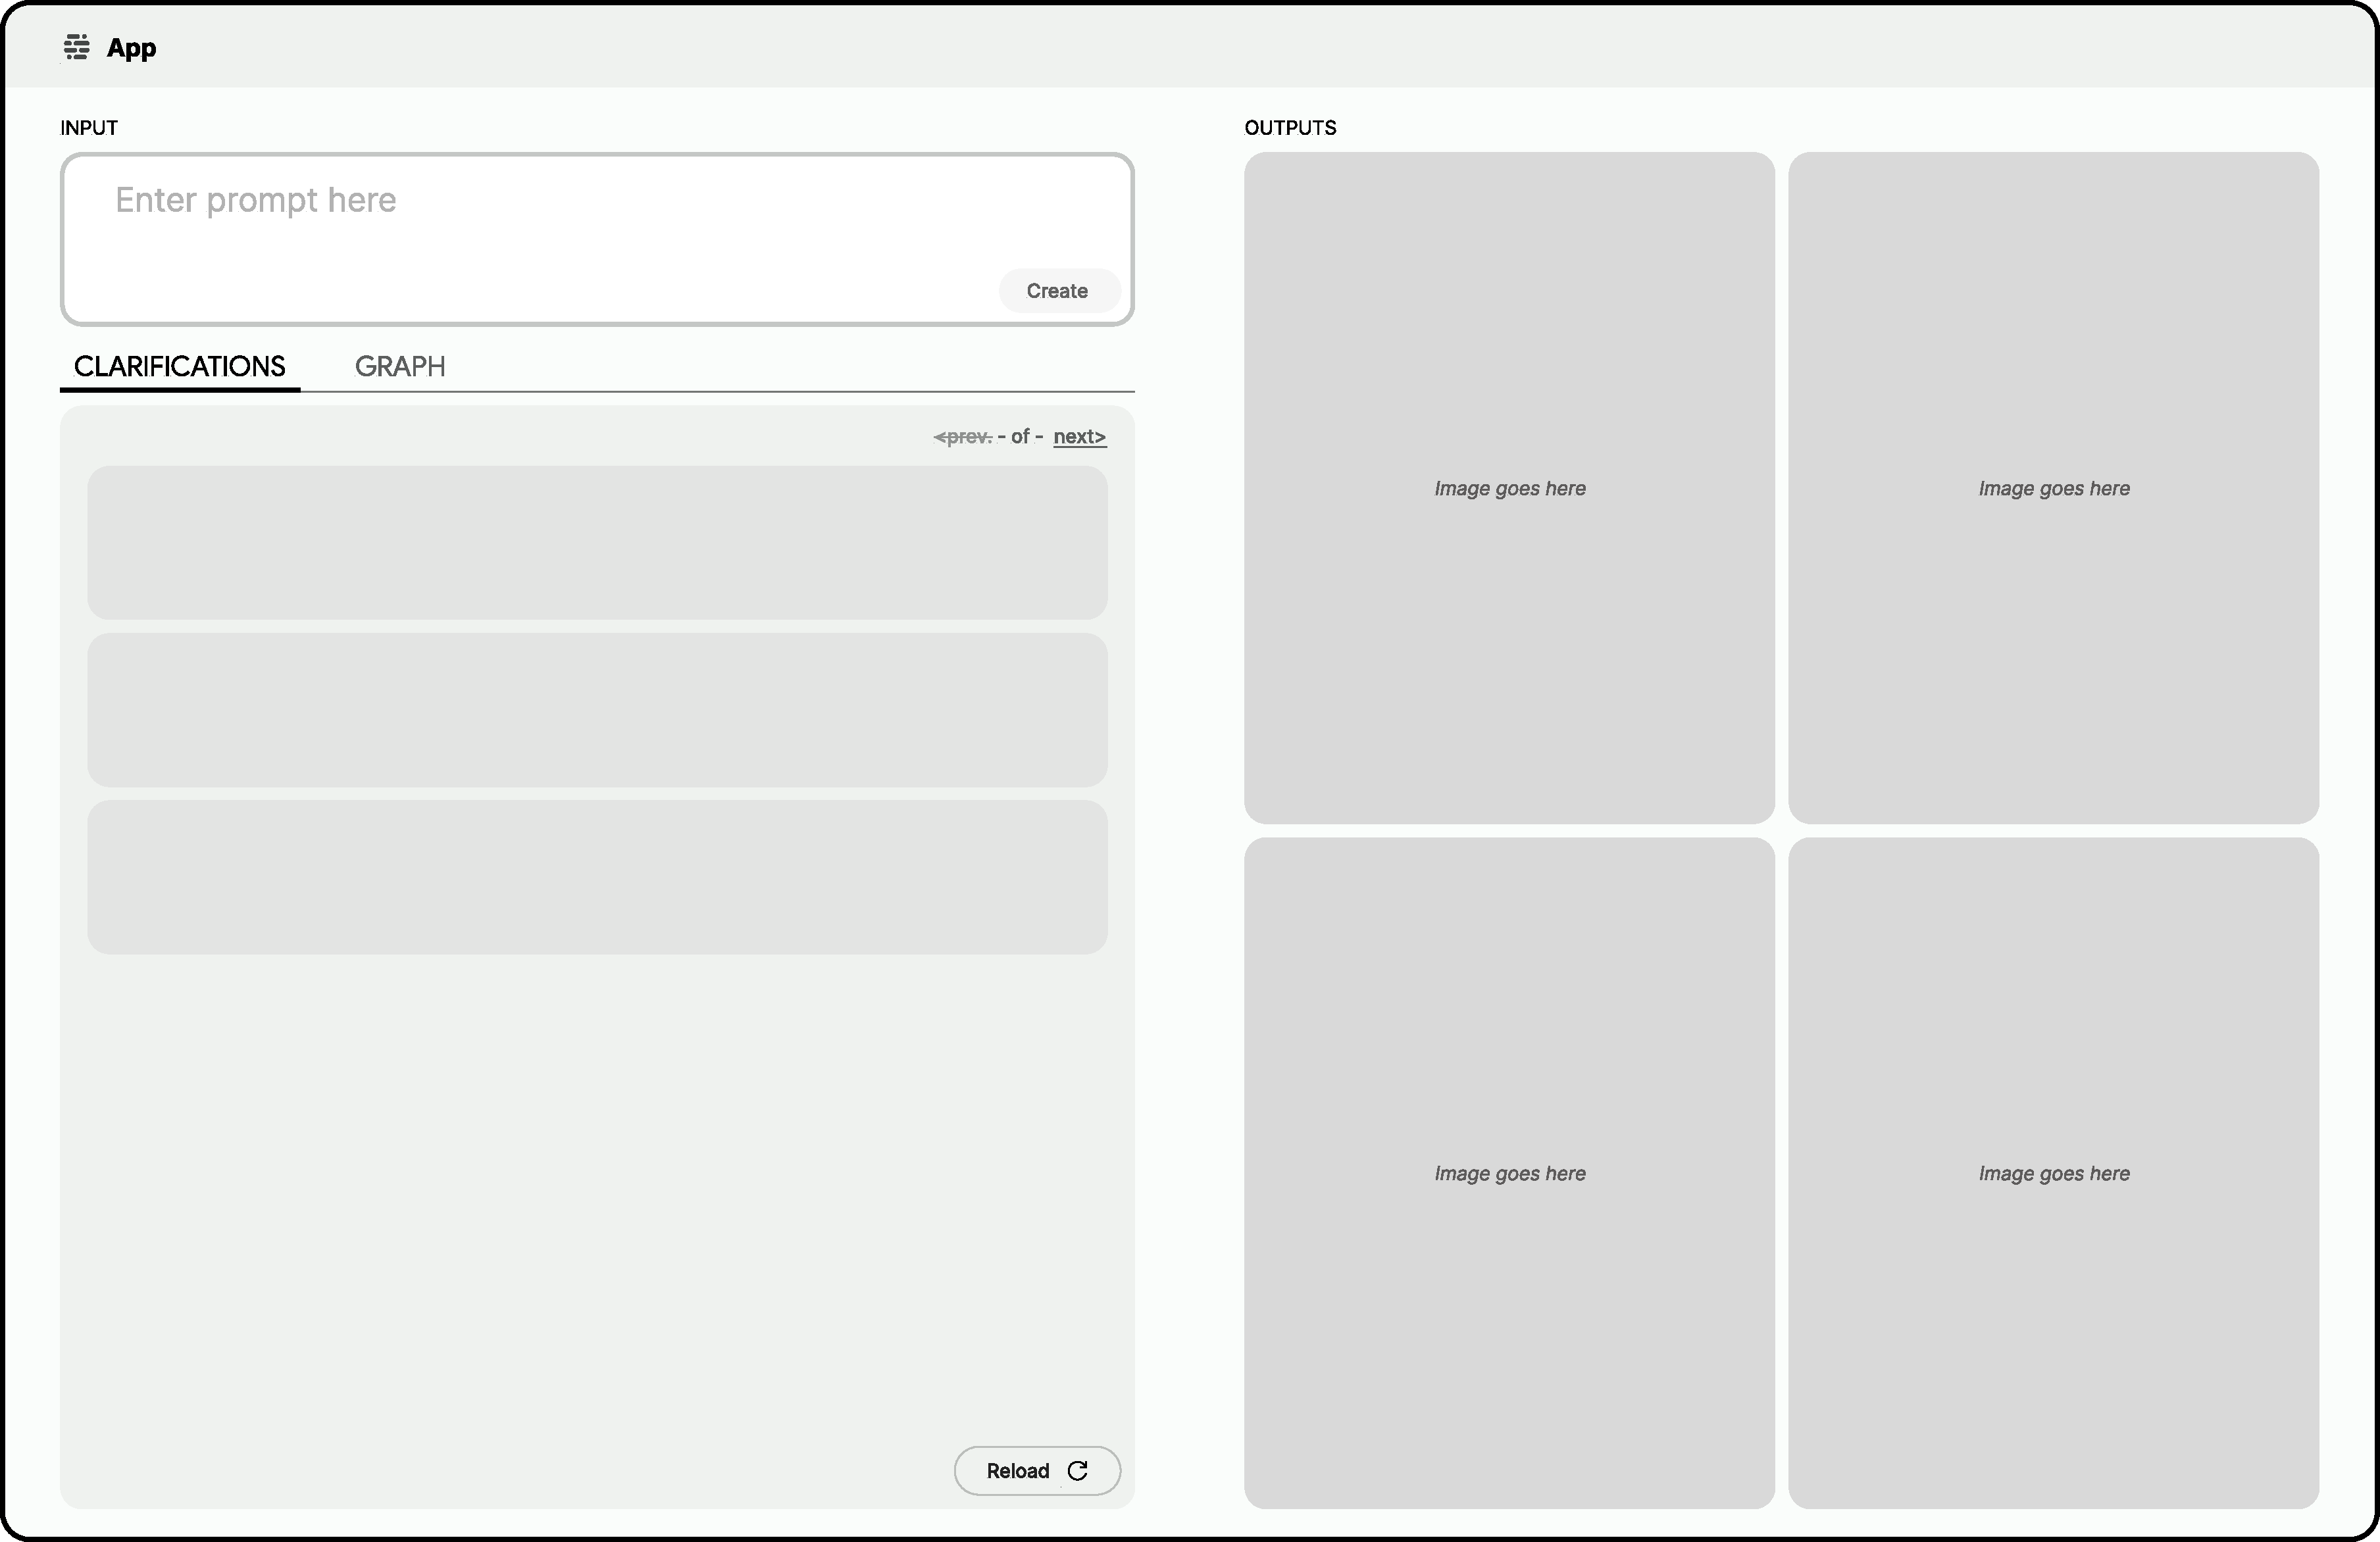
\includegraphics[width=.9\linewidth]{figures/Default.pdf}
    \caption{Default state of a possible interface.}
    \label{fig:interface1}
\end{figure} 

\textbf{2. Output images, with Clarifications} 
Once the user has submitted the prompt and the model has responded, there would be a set of images, as initial outputs from the users prompt. Below the input prompt would be a set of ``Clarifications'' in its populated state. These clarifications would ask the user specific questions that would be necessary to increase the specificity of the prompt, for the model to get a more accurate results aligned to the users intention, or to help the user realise their intention. Options would be given of the highest probability options for each Clarification, but the user could also fill in a totally new option via a free text field. Once answered by selection or text input, the clarifications would be added to the above, primary prompt for regeneration when the user selects. See \Cref{fig:interface2} below as reference.

\begin{figure} [ht!]
    \centering
    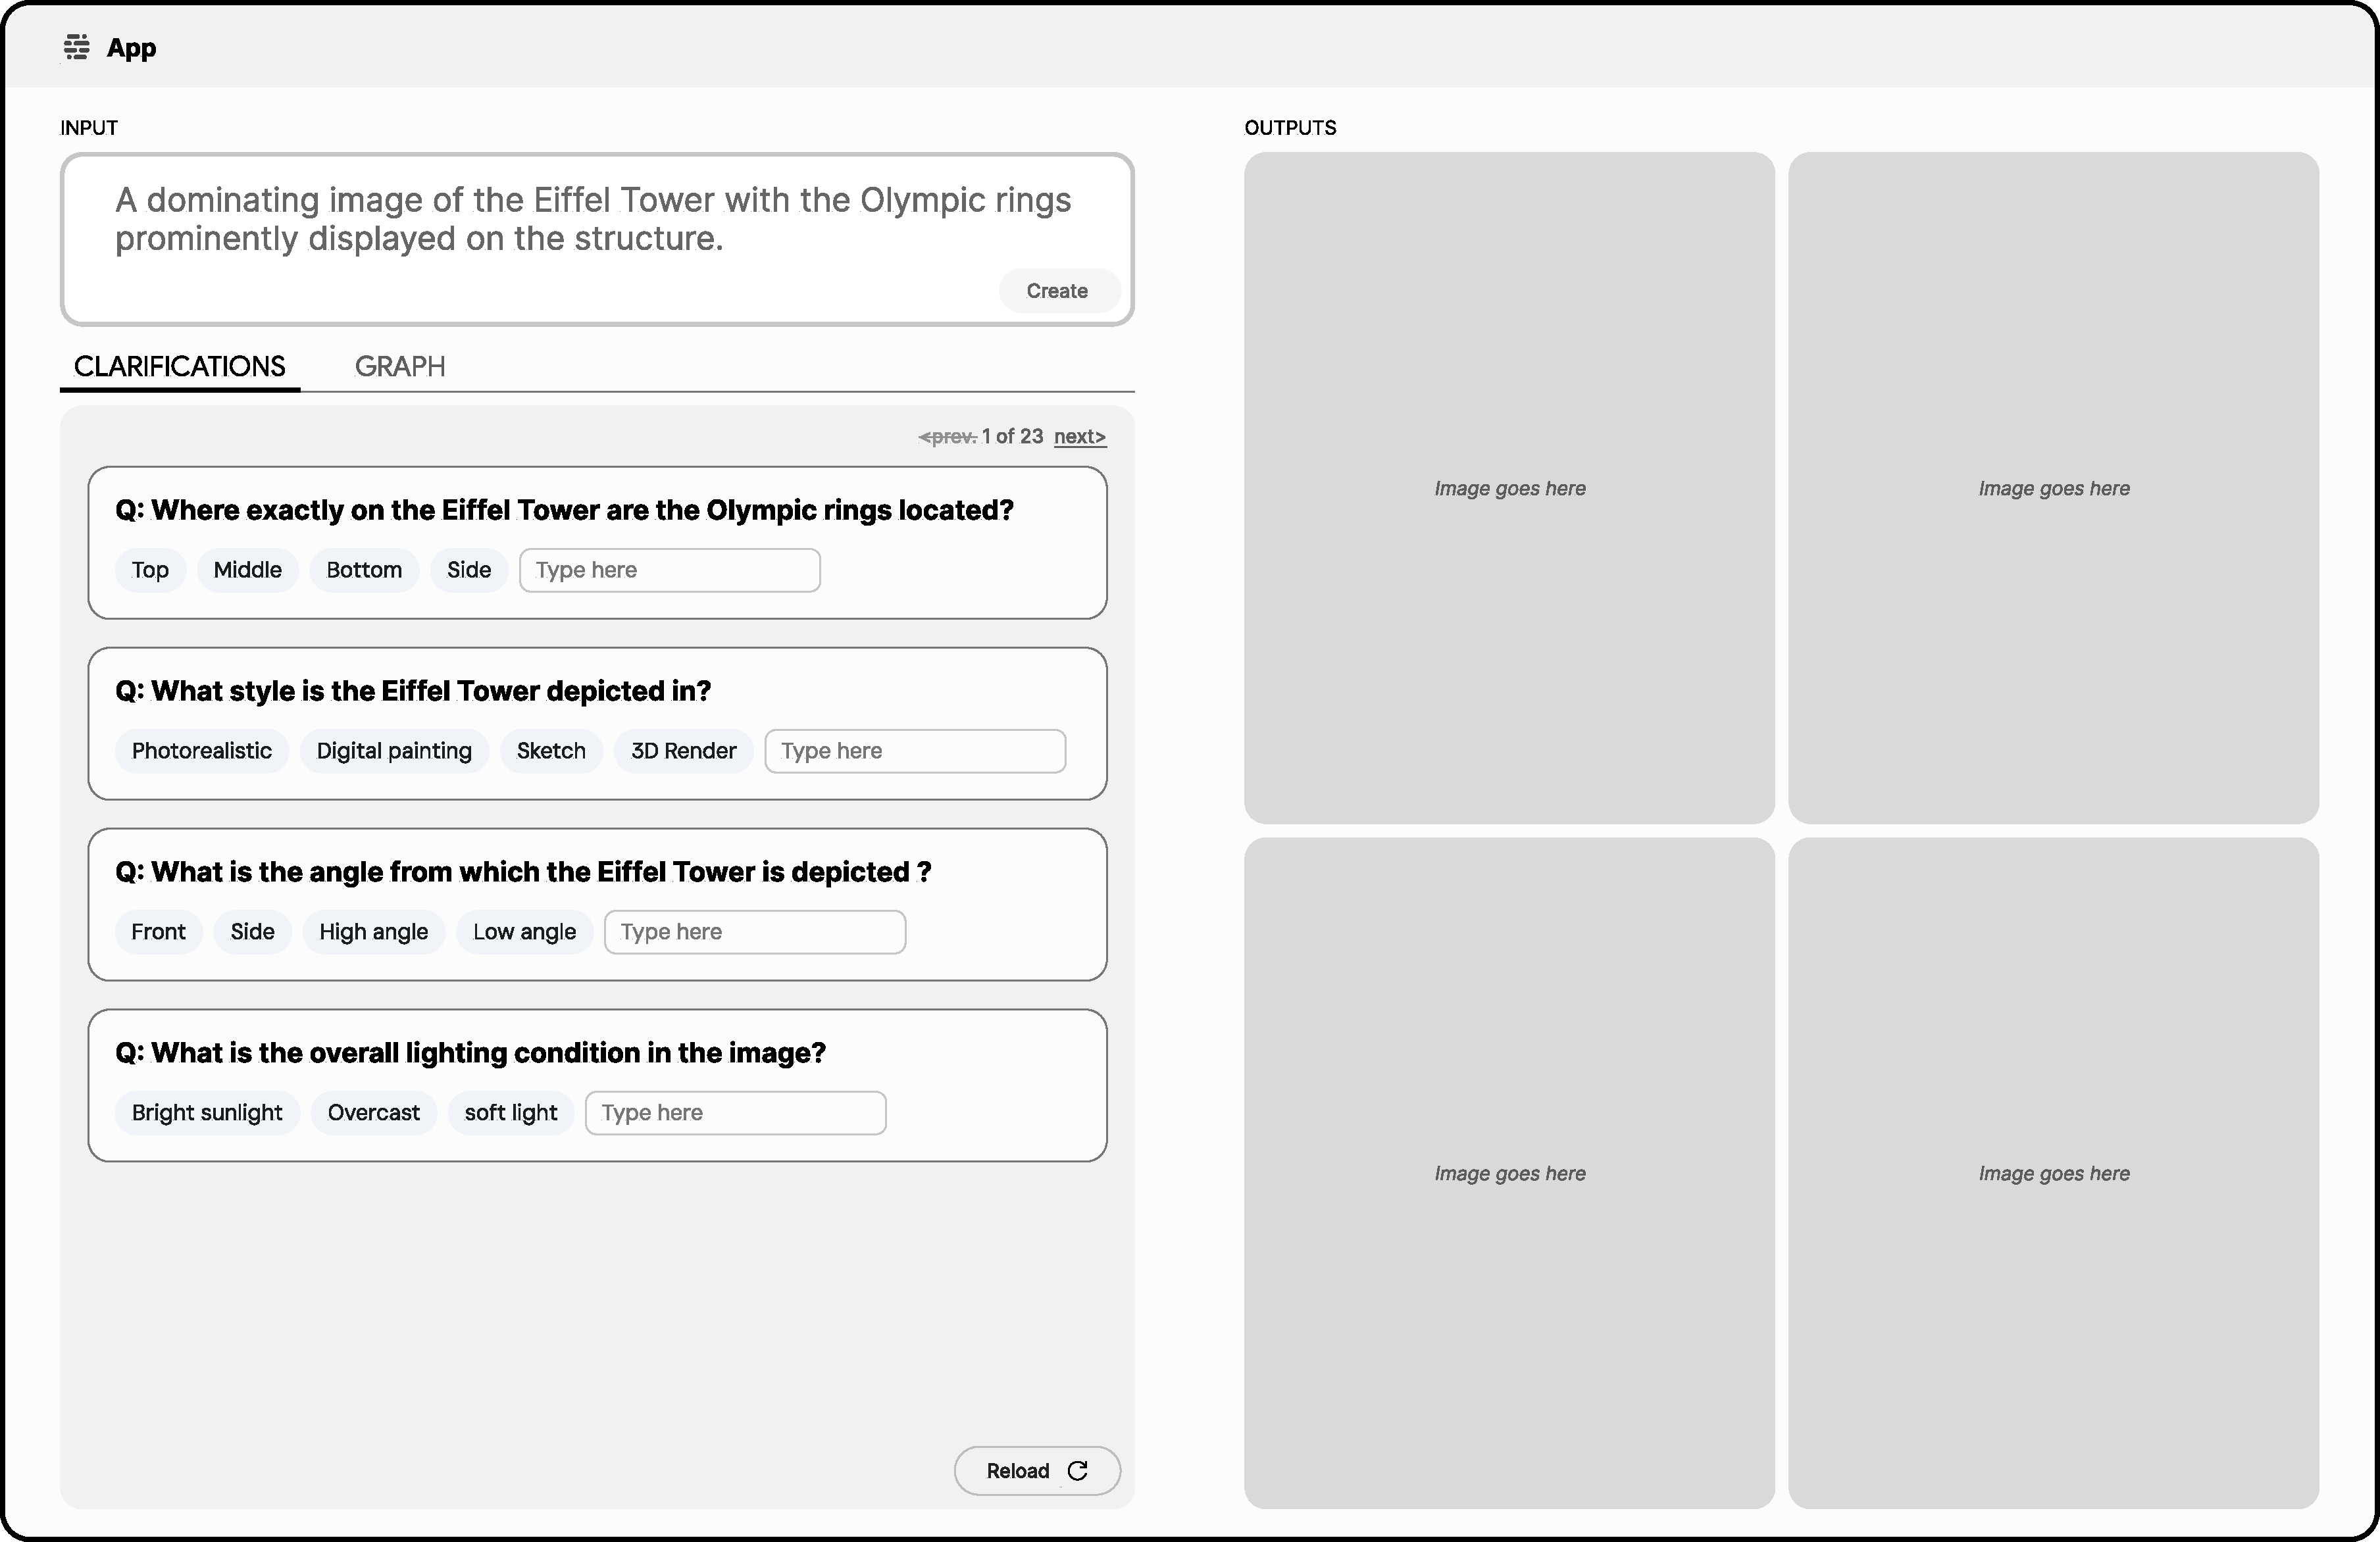
\includegraphics[width=.9\linewidth]{figures/Clarifications.pdf}
    \caption{Interface once prompt has been input with clarifications.}
    \label{fig:interface2}
\end{figure} 

\textbf{3. Graph Entities \& Attributes }
Instead of the clarifications, the user could select to instead view a Graph by clicking  Tab above the clarifications themselves. This graph would  be populated will all Entities from the prompt explicit and implicit visually defined differently (in this diagram by the dotted line surrounds implicit entities, but is a filled line when surrounding explicit entities). The graph layout will be structured, depicting relationships concentrically i.e. "on", "in" or "under" for example, will become child entities, and be displayed within the parent entities' boundary. For example a 'Mug' that has the relationship of 'on' a 'Table' entity, will sit within the boundary of 'Table', as also would a 'Plate' if that had the same child-parent relationship. 

Below the Graph would also be a list of 'cards' (i.e. boxed groups of information), one for each "explicit" or "implicit" entity. Within each card a user could see the status of implicit / explicit, and change this status to confirm or deny its presence. The user could also see a list of "attributes" associated to that entity, which the model has assumed. Each of these attributes could be changed by interacting with a list of alternatives via drop down. These lists are determined in terms of which items and order of items, based on the probability by which the model sees them, ordered with higest first. This probability would be made clear to the user to define the order by seeing the peercentage next to the label. See \Cref{fig:interface3} below as reference.

\begin{figure} [ht!]
    \centering
    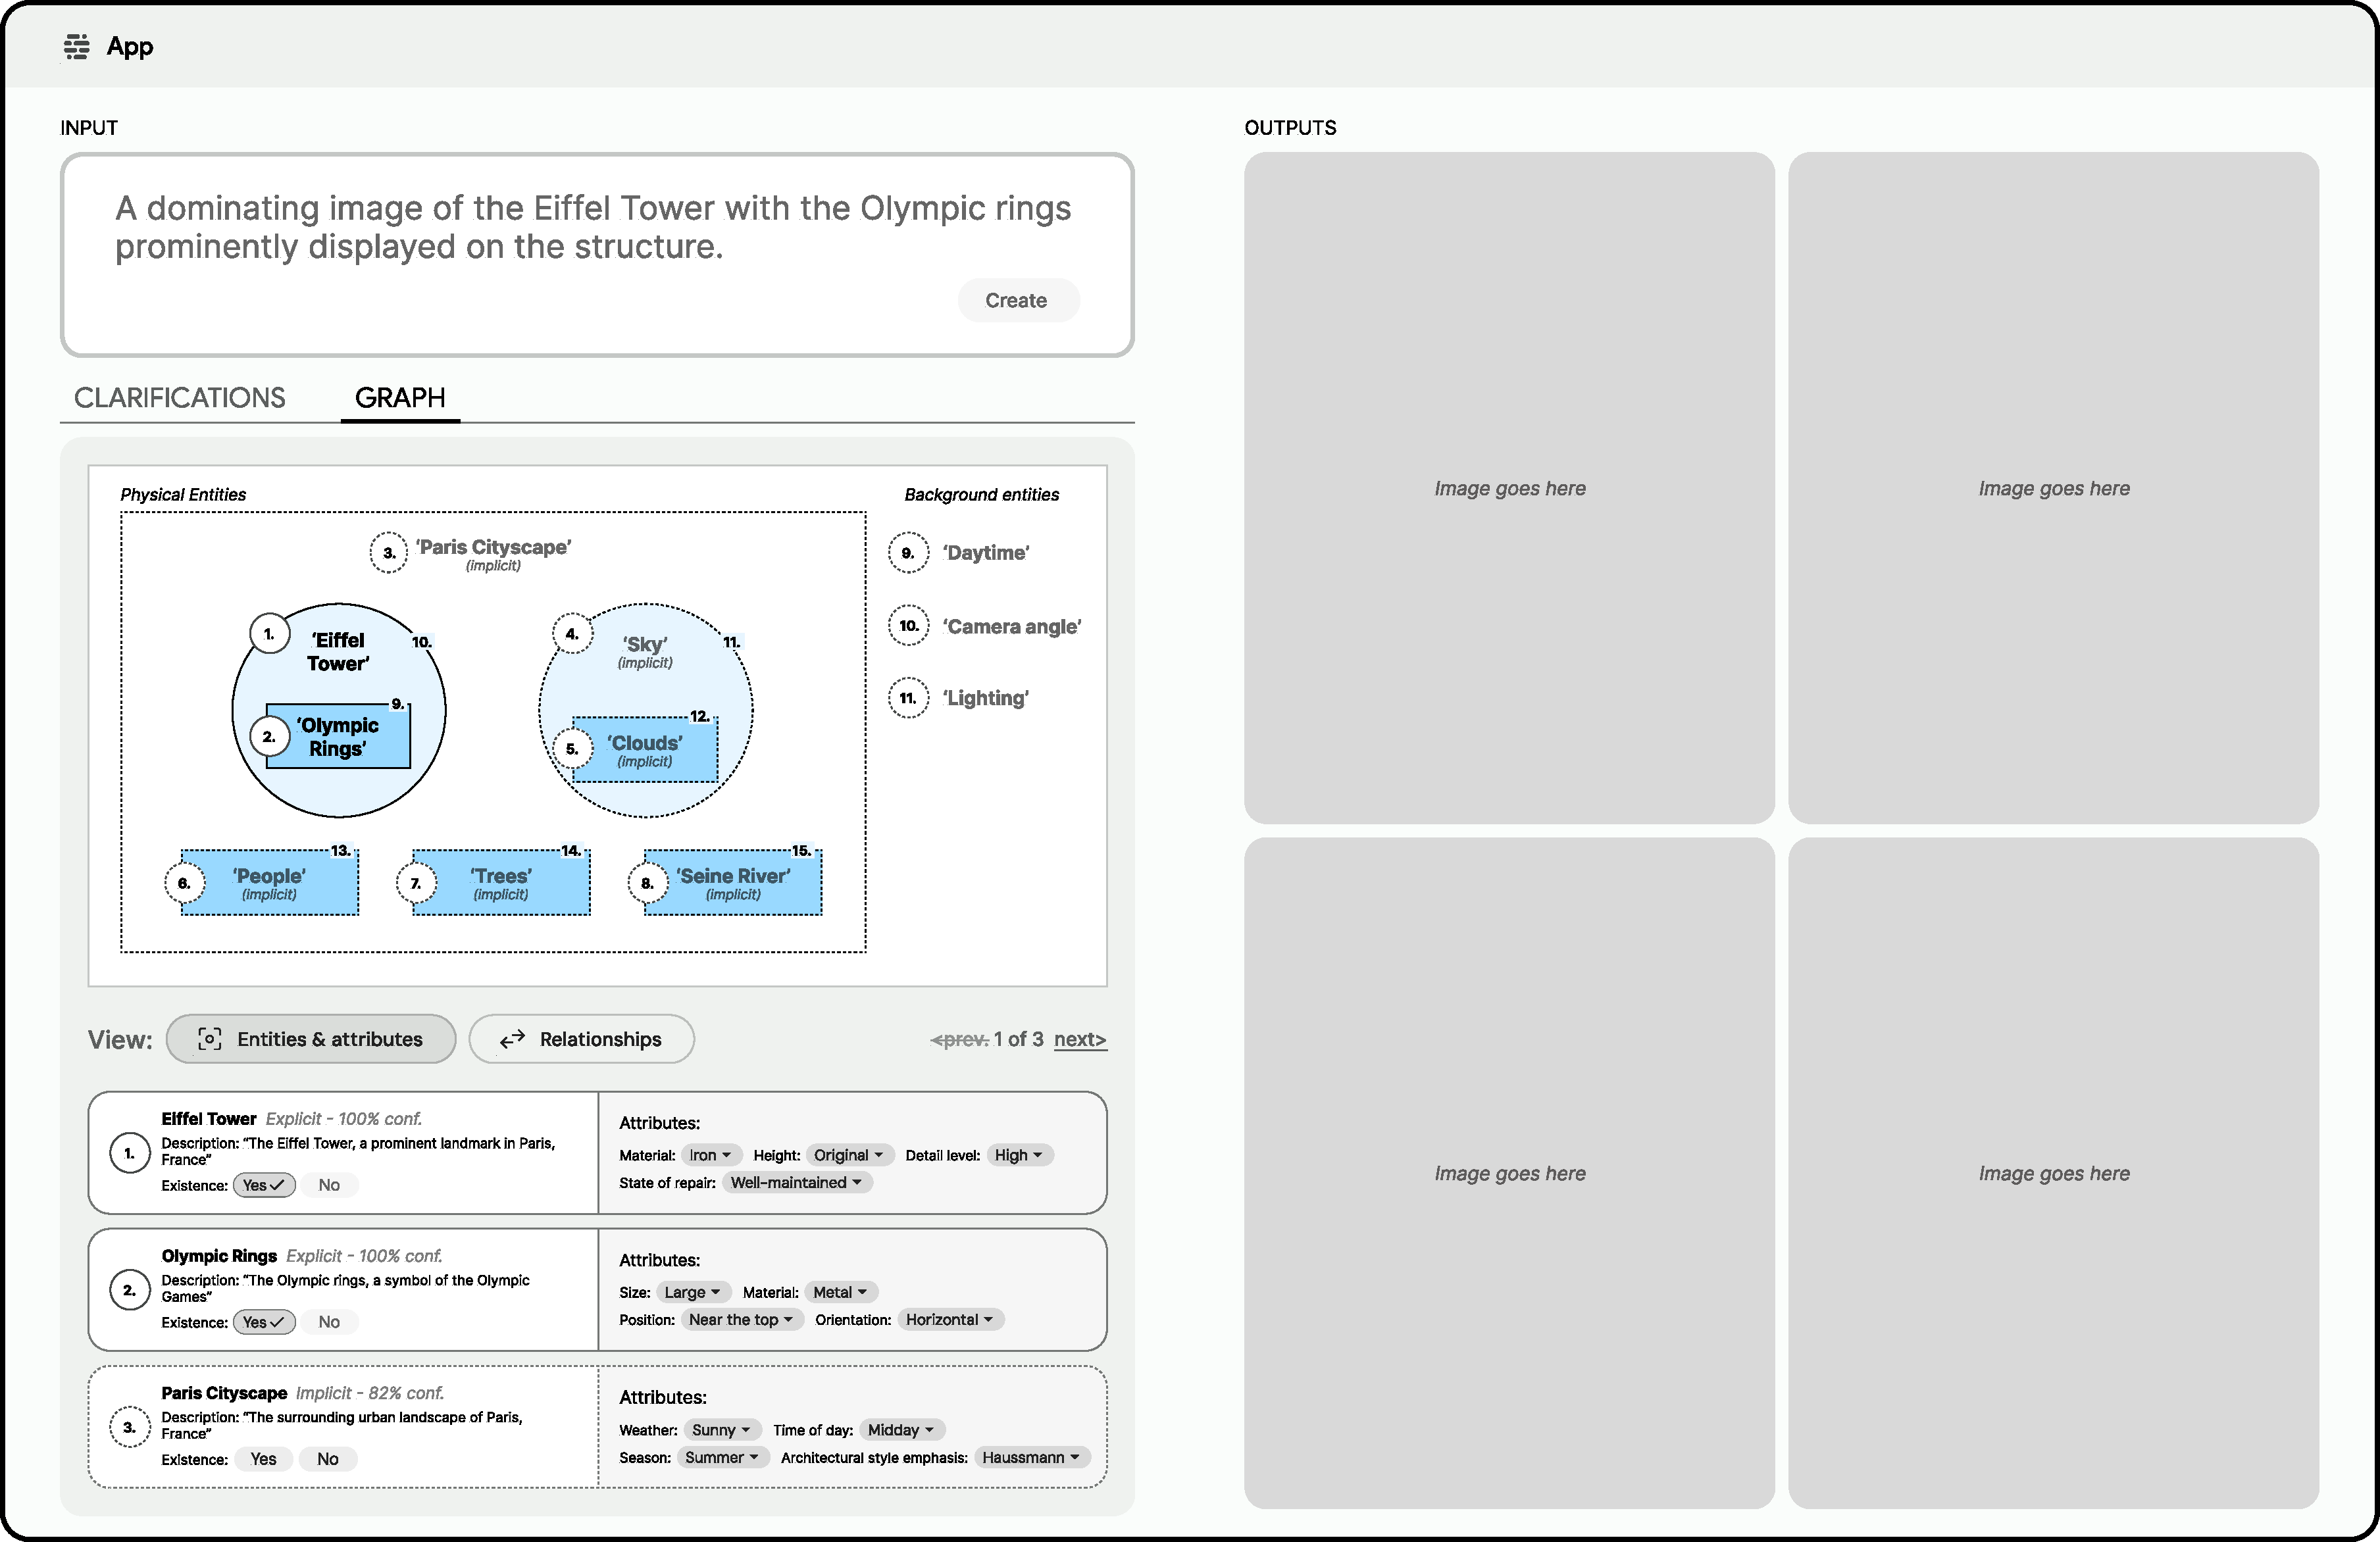
\includegraphics[width=.9\linewidth]{figures/Attributes.pdf}
    \caption{Interface with Graph displaying Entities, with cards below enabling a user to change attributes associated to each entity.}
    \label{fig:interface3}
\end{figure} 

\textbf{4. Graph Relationships} 
The user would also be able to change the state of the Graph and Cards, to instead focus on the relationships between entities, by toggling to "Relations". In this state the user would be able to focus on two specific entities (e.g. 'mug' and 'table'), see the description of the relationship (e.g. 'the mug is sitting on the table') and if desired change the relationship to an alternative (e.g. 'on', changed to 'under') via a drop down of options which the model determined as alternative options ordered by probability, as per attributes. See Figure \Cref{fig:interface4} below as reference.

\begin{figure} [ht!]
    \centering
    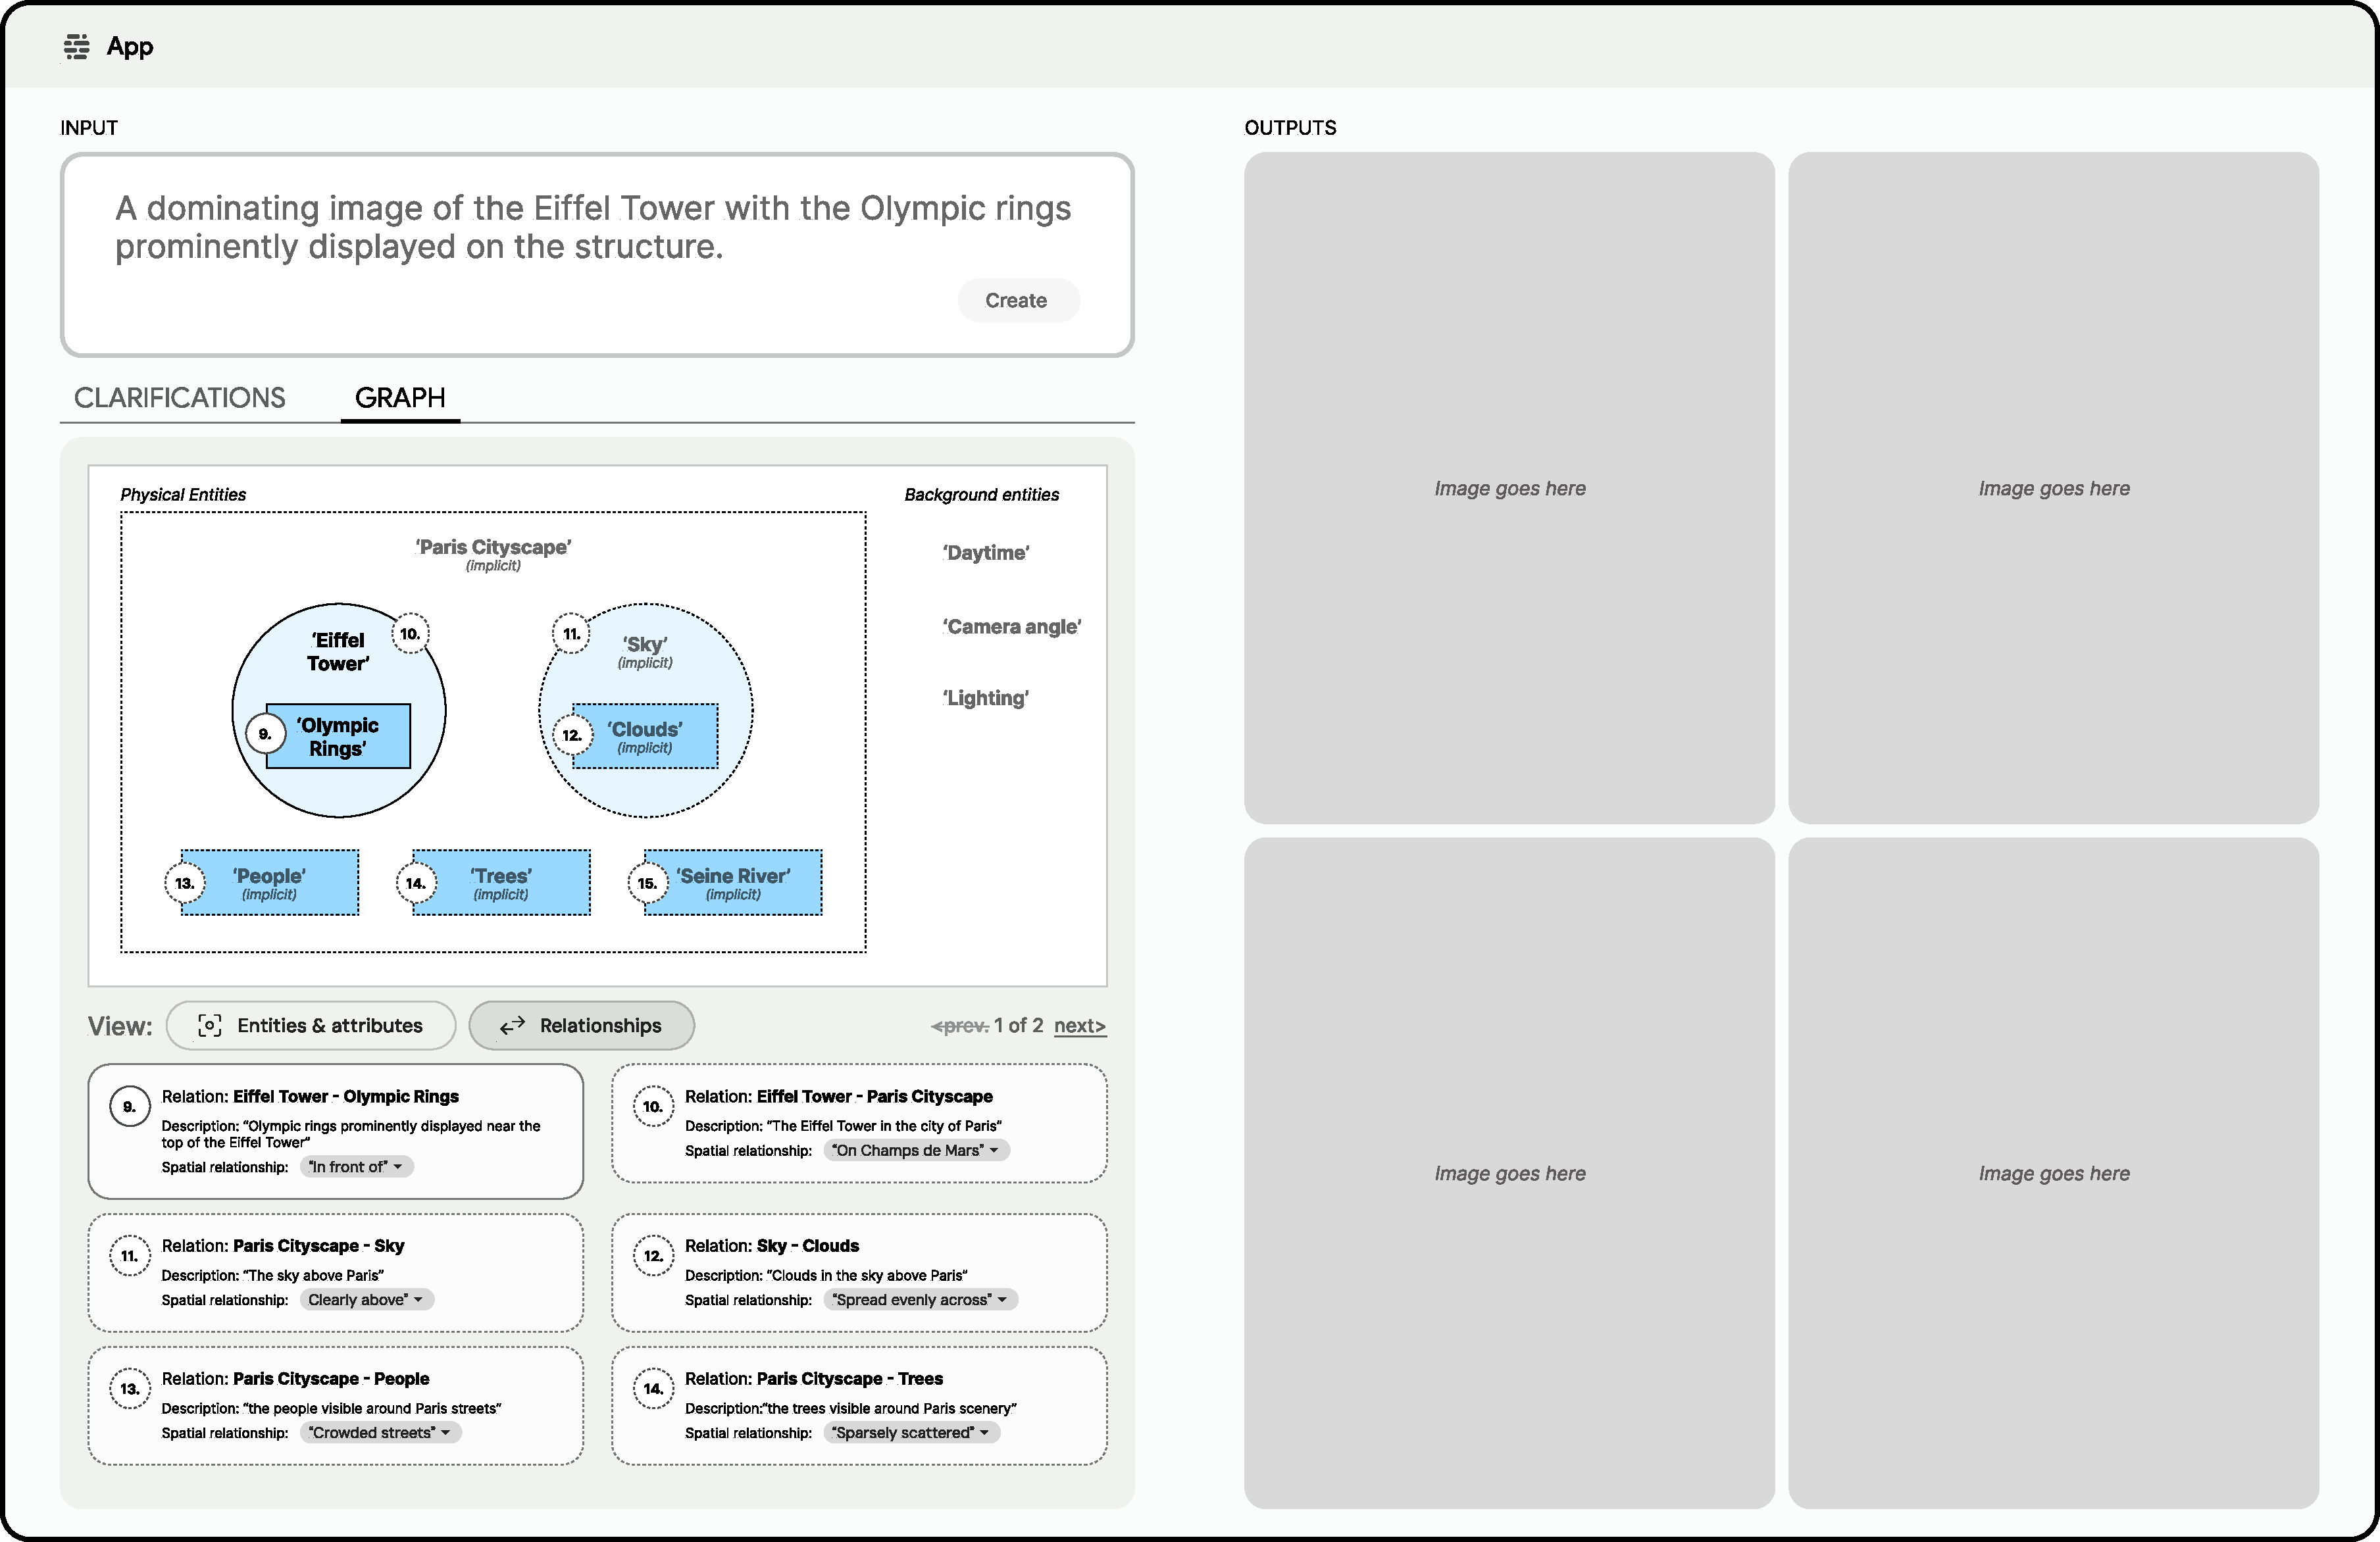
\includegraphics[width=.9\linewidth]{figures/Relations.pdf}
    \caption{Interface with Graph displaying relations between Entities, with cards below enabling a user to change relationships between entities.}
    \label{fig:interface4}
\end{figure} 

Once any of these changes are made the user could initiate a regeneration via the updated prompt to create a new set of output images, which can then be further refined via the same method. 


\section{Details on user studies for the agent interface}
\label{user_study}
Below we describe the exact guideline definitions we shared with the user for a user study.

\subsubsection{Hypothesized Frustrations}
We presented participants with the following hypothesized frustrations related to T2I model usage:
\begin{enumerate}
\item \textbf{Prompt Misinterpretation:} The model misunderstands complex relationships between entities in the input prompt.
\item \textbf{Many Prompt Iterations:} The model does not immediately generate what the user intends, requiring numerous iterative changes to the input prompt.
\item \textbf{Inconsistent Generations:} The model reinterprets the input prompt differently between iterations, causing unwanted changes in the generated images.
\item \textbf{Incorrect Assumptions:} The model makes incorrect assumptions or no assumptions when encountering gaps in the details provided in the input prompt, leading to undesired outputs.
\end{enumerate}

Explanations of terms were given to users of: 
\begin{enumerate}
\item "Entities" are single items that are intended to be in the image e.g. "Cat" and "Ball", from "make a sketch of a Cat playing with a Ball"
\item "Prompt" means the text written to communicate the intended output image e.g. the sentence "make a sketch of a Cat playing with a Ball" is the "Prompt", also known as "Input" 
\item "Iterations" are each set of different image outputs by the model, taken from a different input, or even the same input just regenerated
\end{enumerate}

The question asked for each Frustration were: "Please score the below frustrations (or issues) that could be related to Text to Image AI Generation"."Rank in terms of how much they relate to your current usage, with your most commonly used model or app." 




\subsubsection{Hypothesized Features}
We proposed the following features as potential solutions to address the identified frustrations:
\begin{enumerate}
\item \textbf{Clarifications:} The model would ask specific clarifying questions about uncertainties in the prompt.  These details would then be incorporated into subsequent iterations. For example: "Is the cat playing with: 1. a ball of wool, or 2. a tennis ball?"
\item \textbf{Graph of Prompt Entities:}  A visual representation of all entities in the prompt as a graph, allowing users to see and edit attributes of each entity.  E.g., seeing that the model has assigned "round," "small," and "wooden" as attributes to "table" and allowing the user to change them to "square" and "metal."
\item \textbf{Graph of Prompt Relationships:} A visual representation of relationships between entities in the prompt, allowing users to see and edit these relationships. E.g., seeing that "donut" is "next to" "coffee" and allowing the user to change the relationship to "on top of."
\end{enumerate}

The questions asked for each feature were: 
\begin{enumerate}
\item "How likely this feature is to help your current workflow if you had it now?". With response options of: "Very unlikely to help", "Unlikely to help", "Could help", "Likely to help", "Very likely to help". 
\item "How soon would this feature deliver value to your work?" with response options of: "Very soon / immediately", "Sometime, "Not very soon".
\end{enumerate}

Image references were given for each Feature as listed out below:

\begin{enumerate}
\item \textbf{Clarifications:} 
\begin{figure} [H]
    \centering
    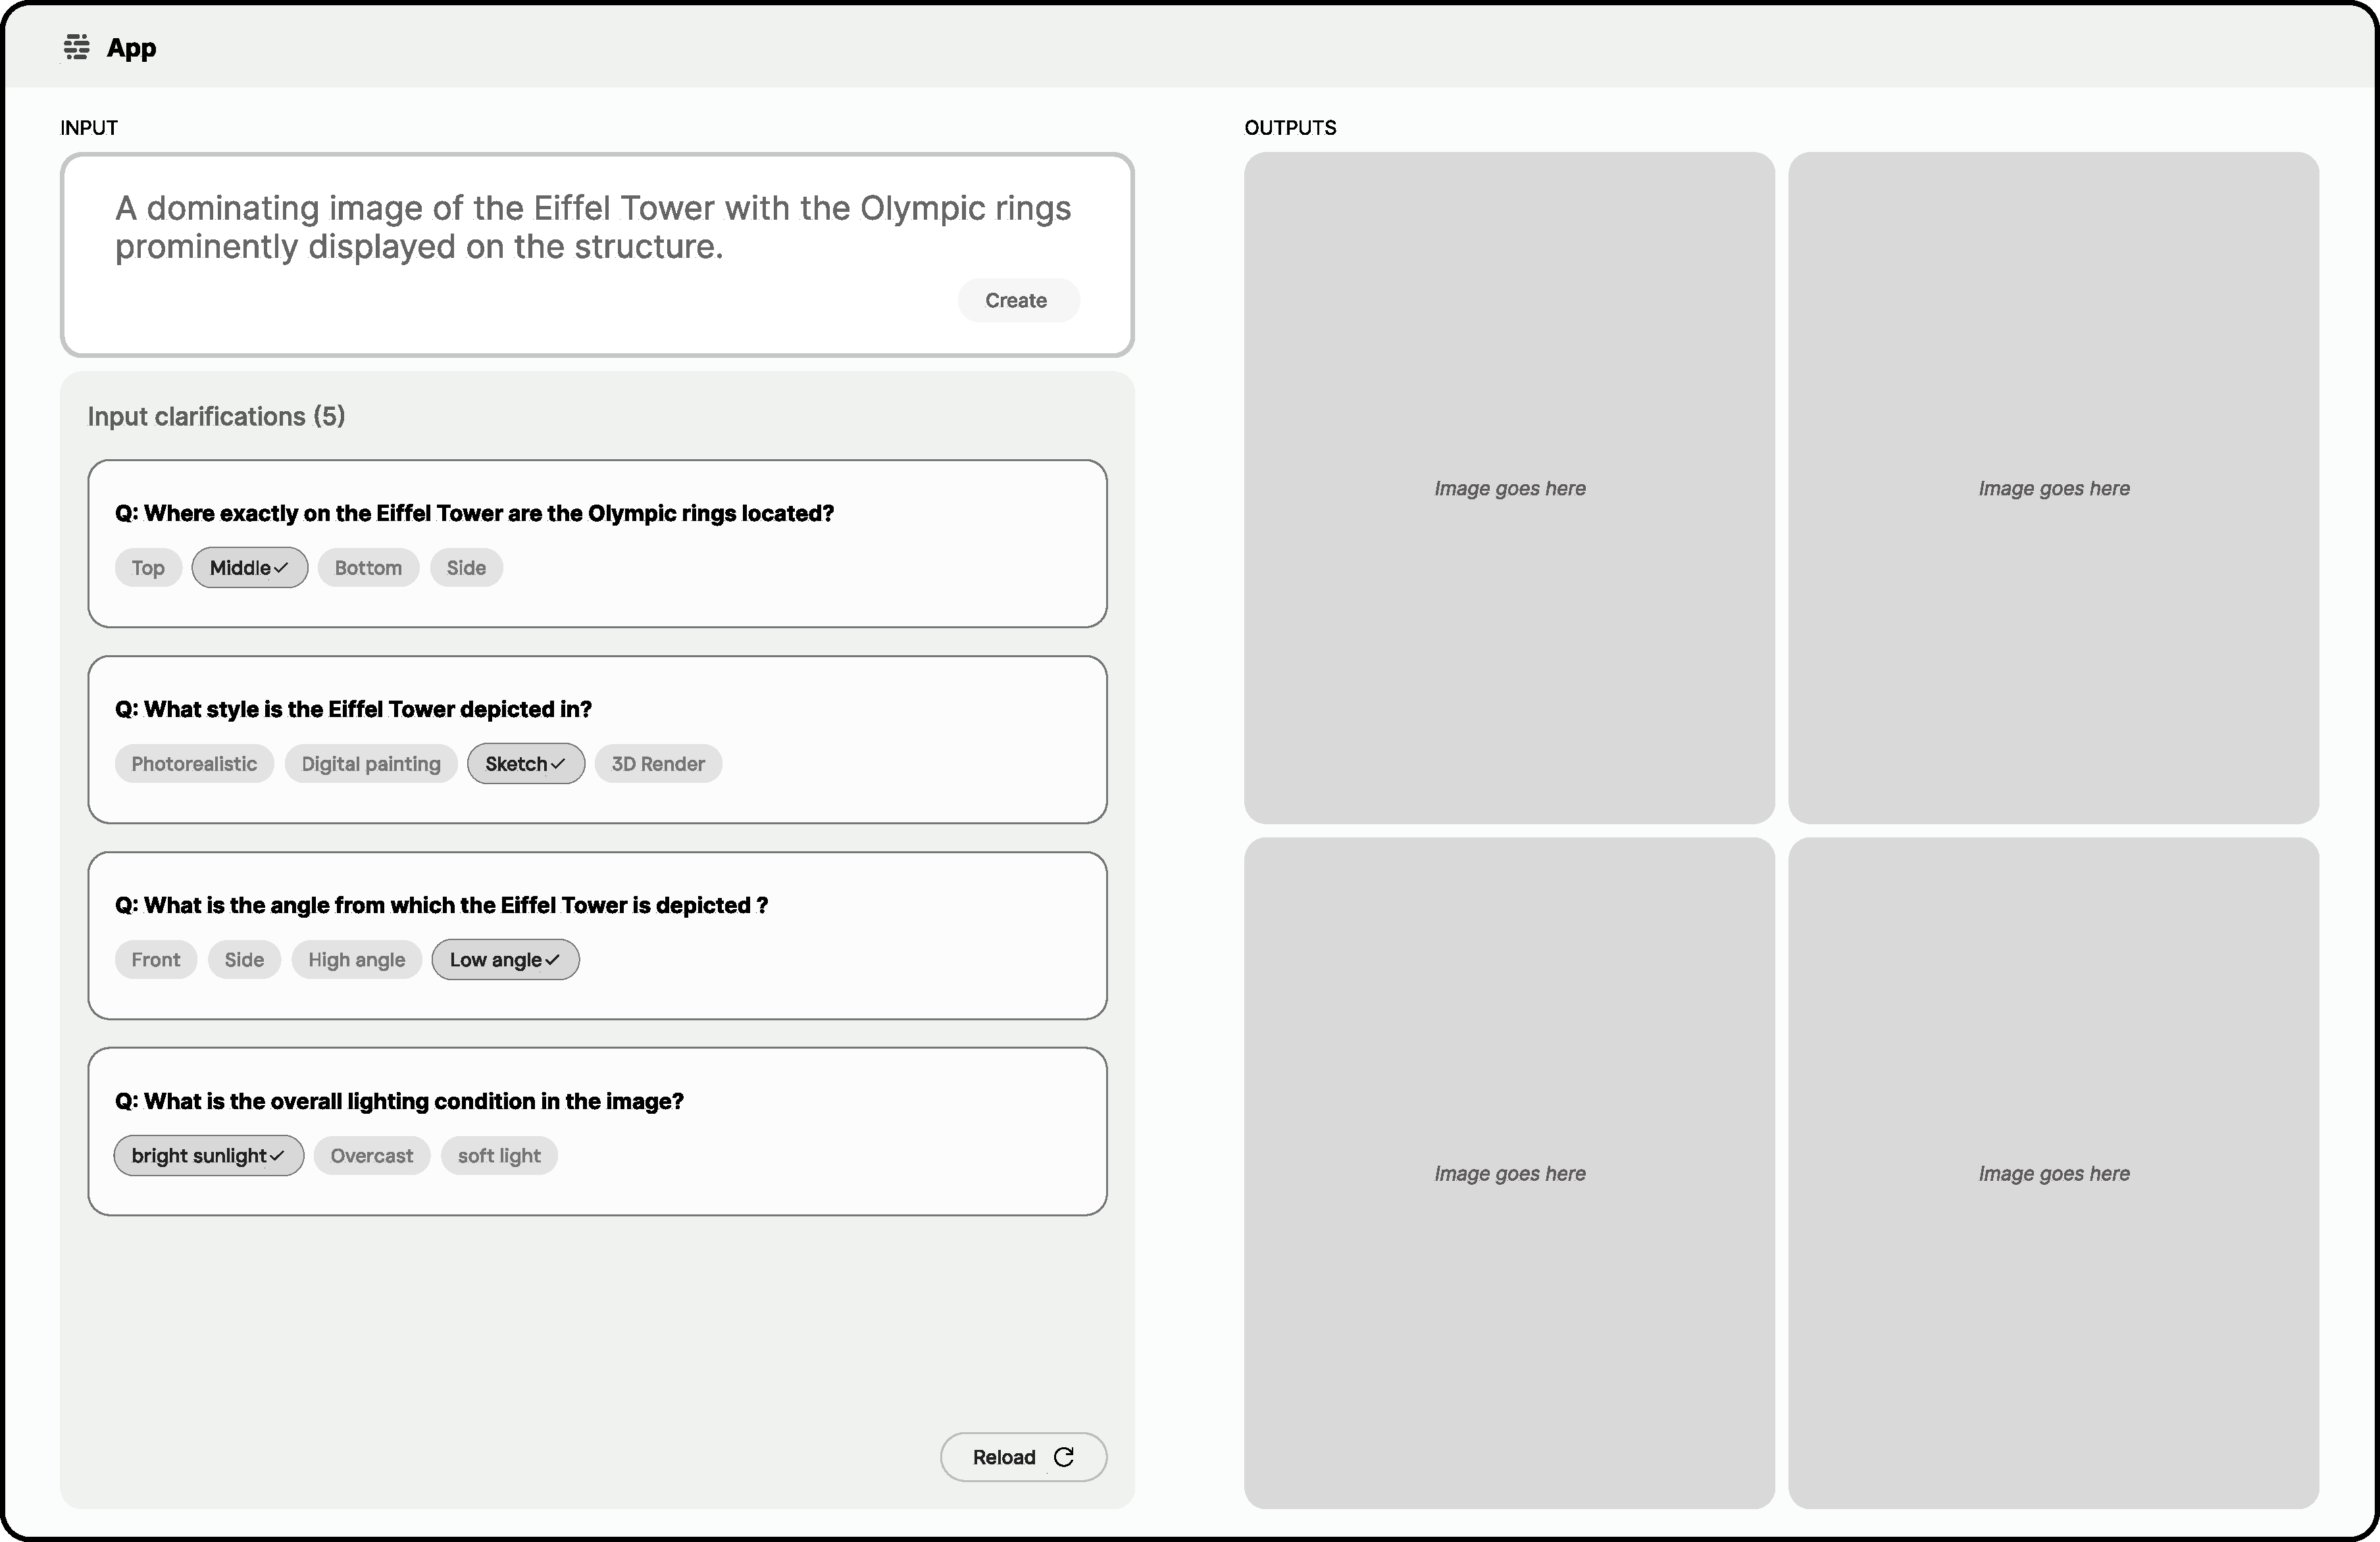
\includegraphics[width=.9\linewidth]{figures/F1_Questions.pdf}
    \caption{Stimulus image in the survey to test the Model clarifications feature.}
    \label{fig:interface-human}
\end{figure} 

\clearpage
\item \textbf{Graph of Prompt Entities:}  
\begin{figure} [H]
    \centering
    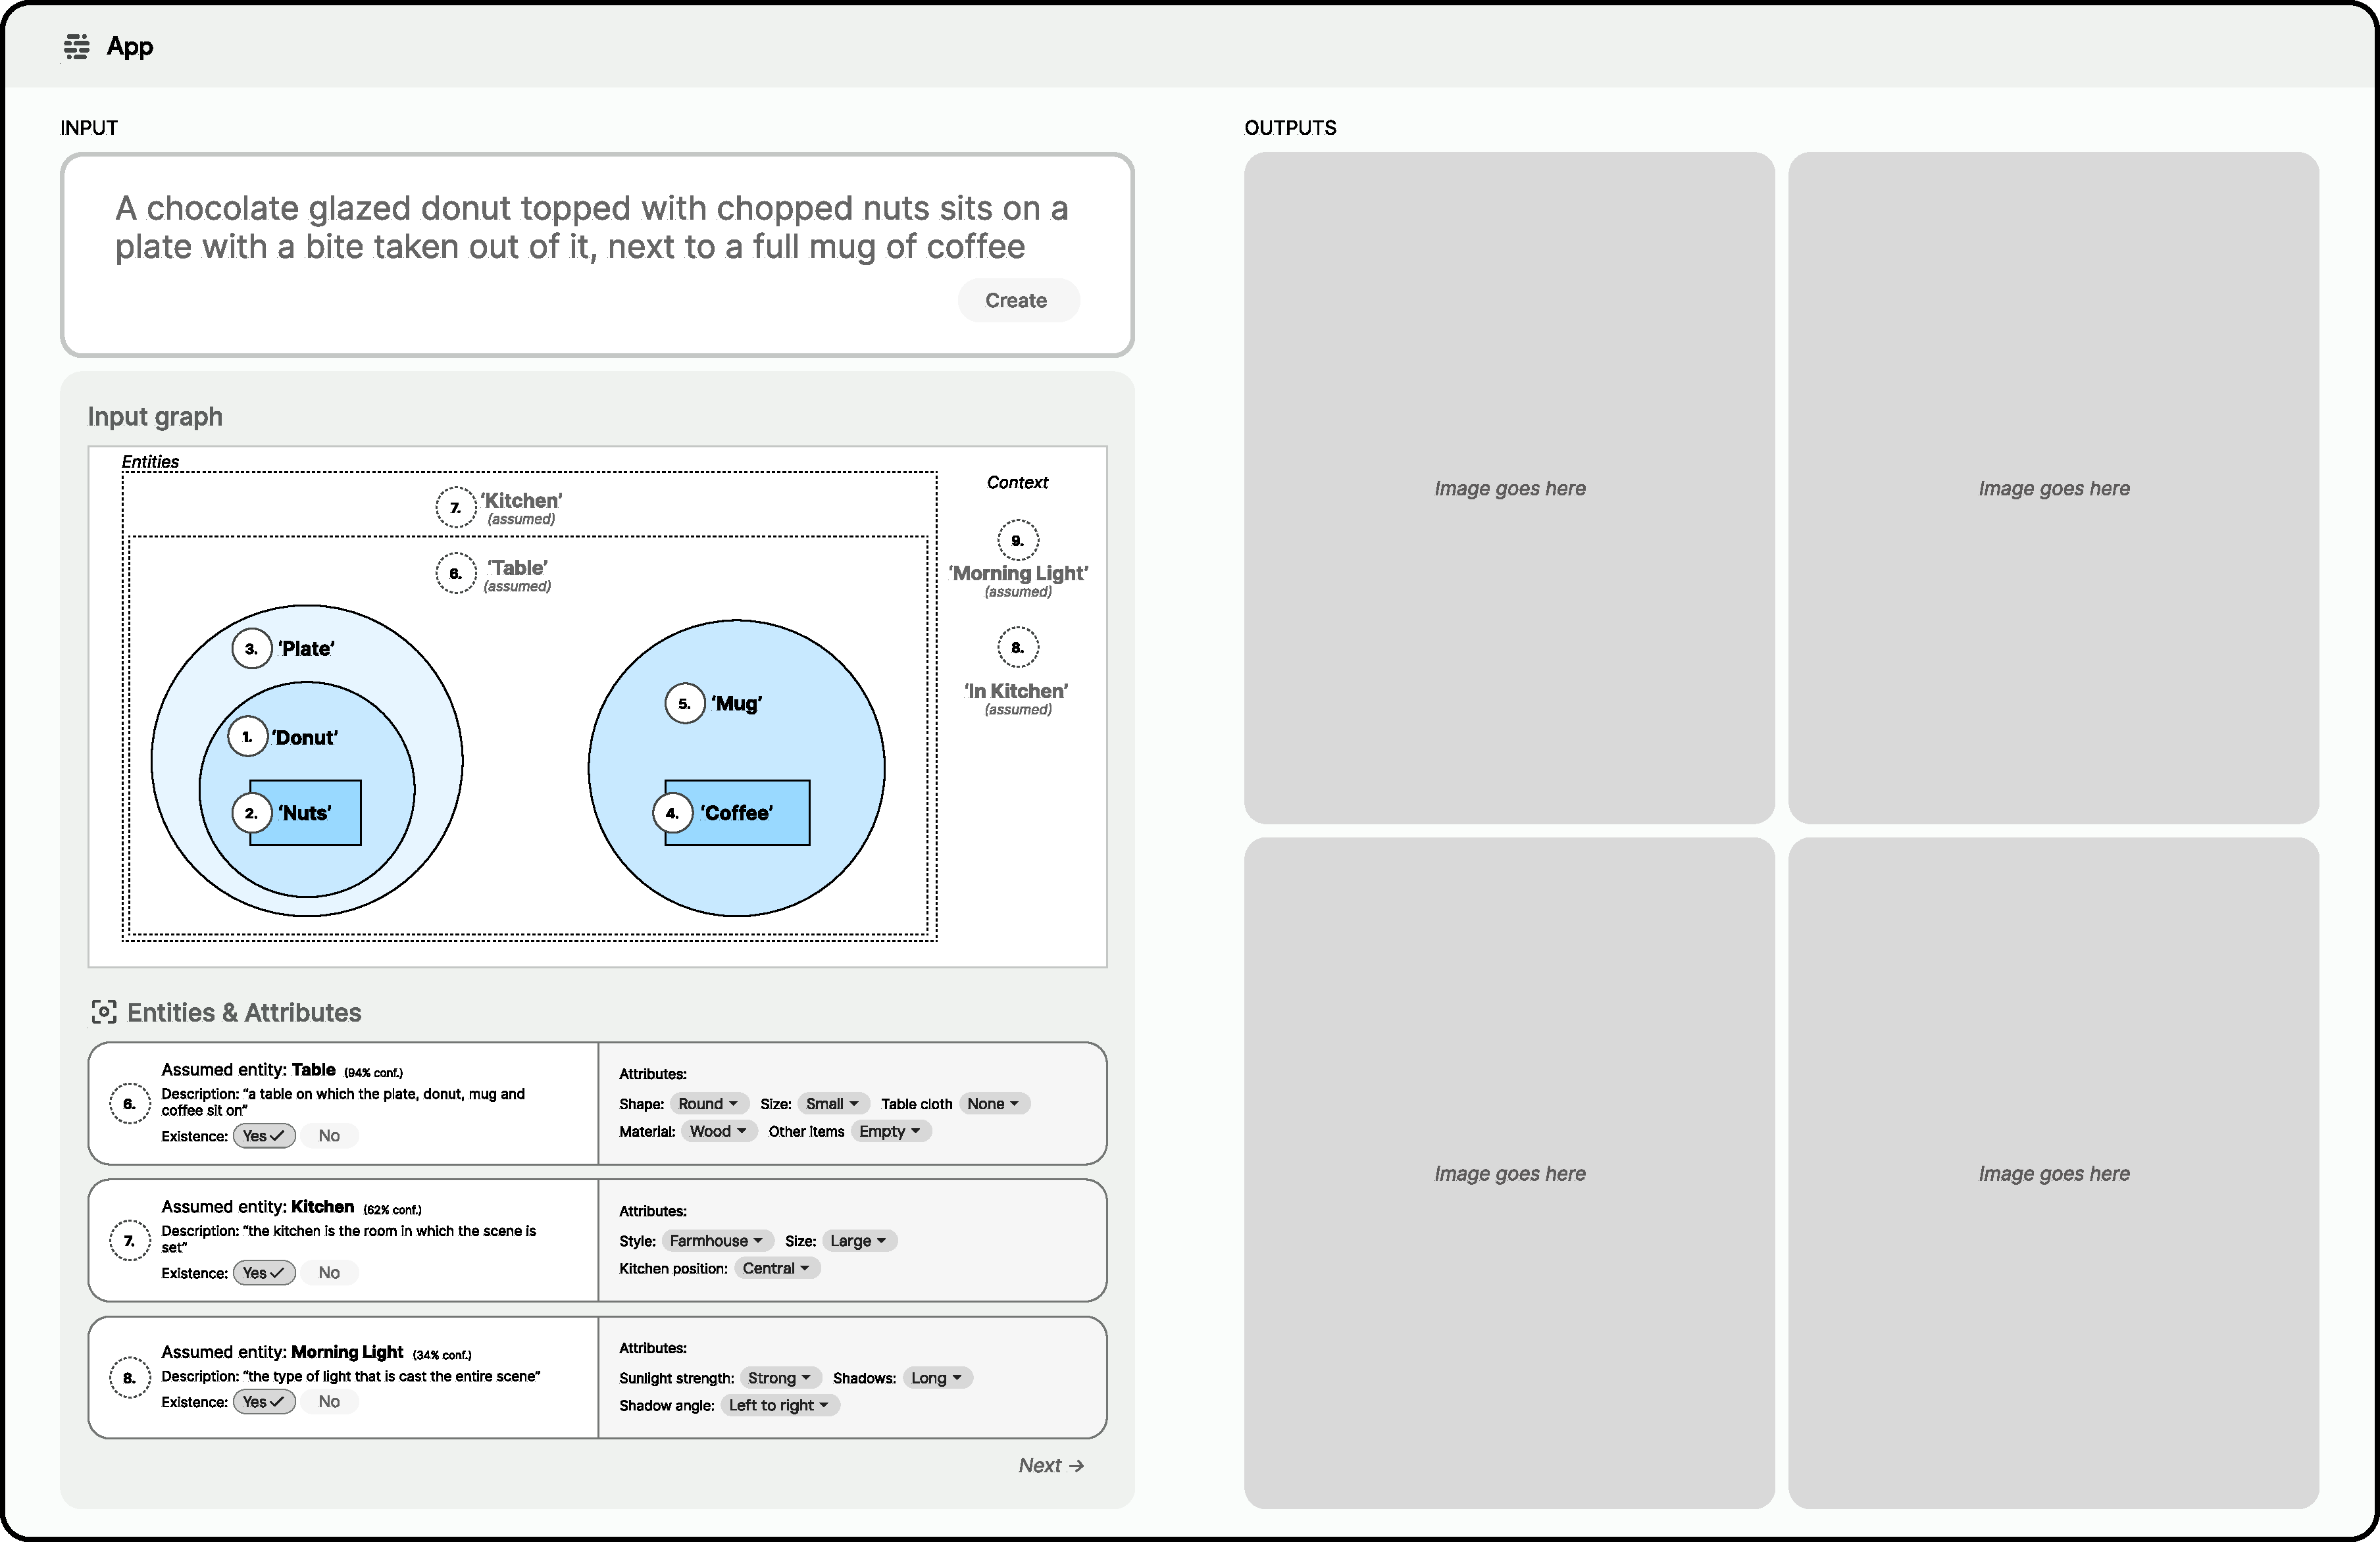
\includegraphics[width=.9\linewidth]{figures/F2_Graph.pdf}
    \caption{Stimulus image in the survey to test the Model Graph of Entities and Attributes feature.}
    \label{fig:interface-human2}
\end{figure} 

\item \textbf{Graph of Prompt Relationships:} 
\begin{figure} [H]
    \centering
    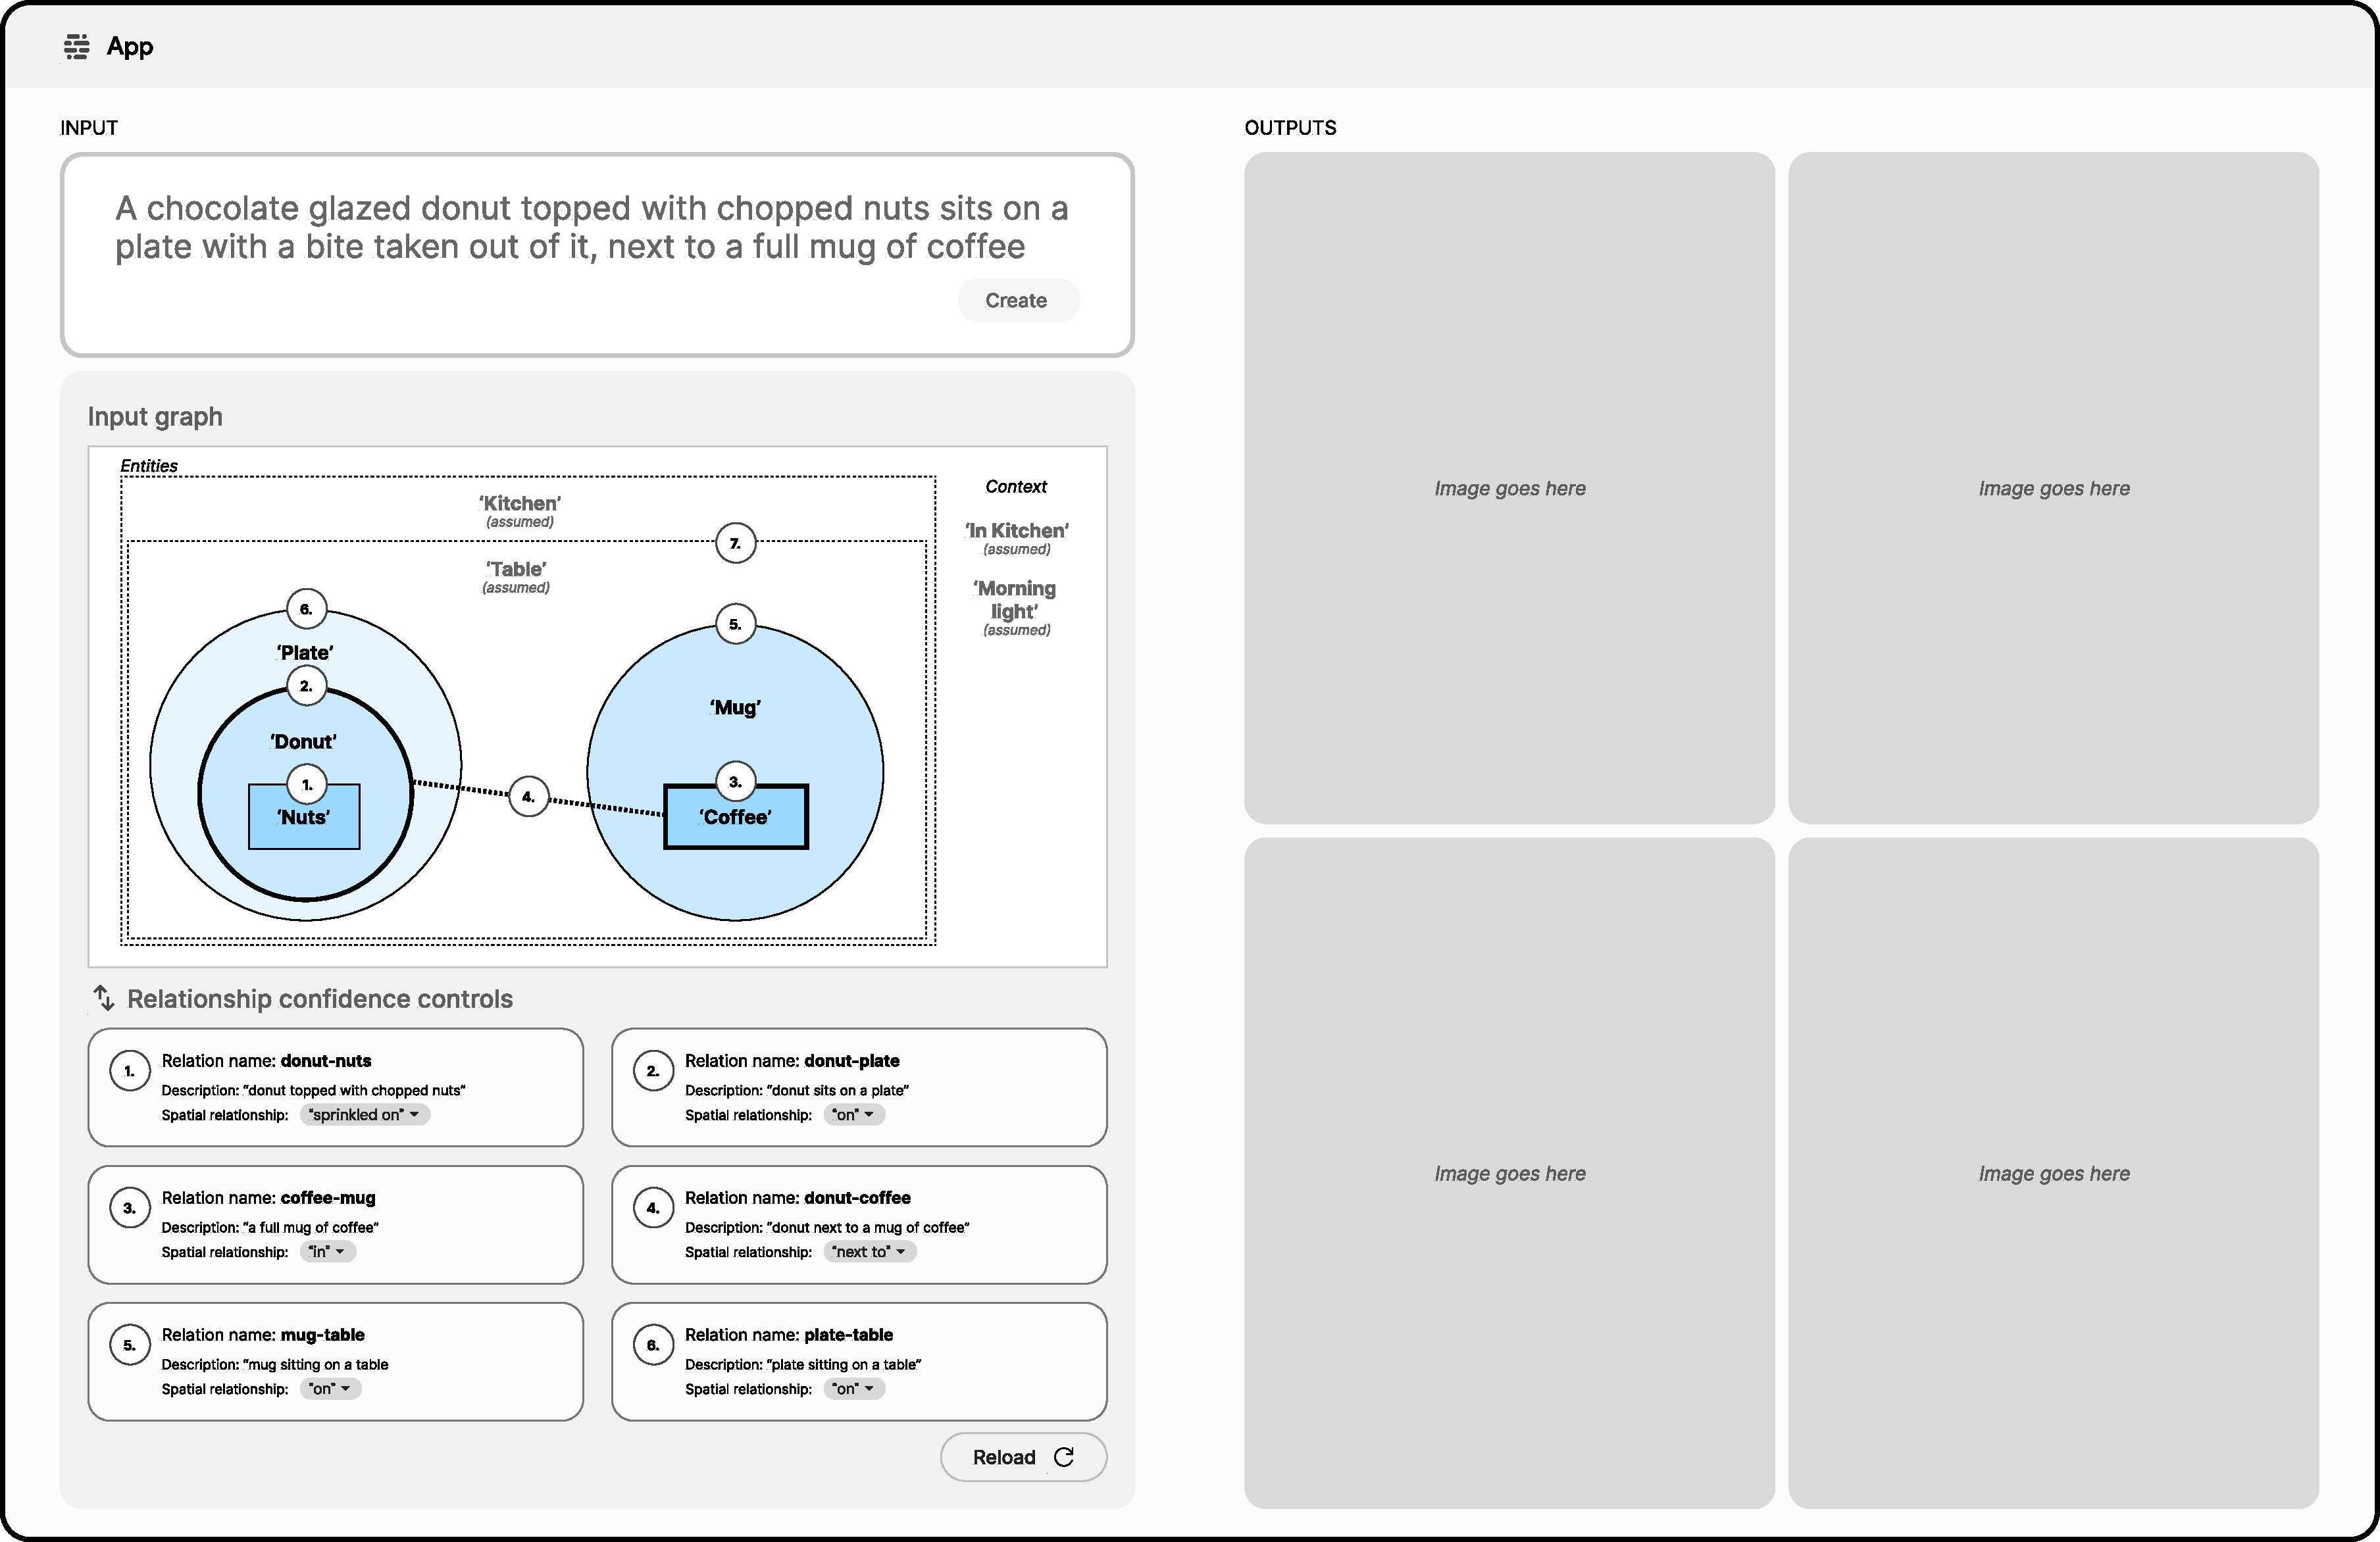
\includegraphics[width=.9\linewidth]{figures/F3_Relations.pdf}
    \caption{Stimulus image in the survey to test the Model Graph of Entity Relations feature.}
    \label{fig:interface-human3}
\end{figure} 

\end{enumerate}

\subsubsection{Human Study Results}
\Cref{tab:t2i_frequency} details the T2I usage frequency of the human subjects. \Cref{table_frustration1} shows the percentage of human subjects that reported different kinds of frustrations in their experience of using T2I. \Cref{table_frustration2} summarizes the results on expected speed of value delivered from different features of our agent prototypes. These results highlight the impact of our contributions.
\begin{table}[h]
\caption{Breakdown of the T2I usage frequency of the 143 participants recorded}
\centering
\label{tab:t2i_frequency}
\begin{tabular}{lrr} 
\toprule
\textbf{Usage Frequency} & \textbf{No. of participants} & \textbf{(\%)} \\
\midrule
Many times a day & 13 & 9.1 \\ 
Many times a week & 44 & 30.8 \\
At least once a week & 36 & 25.2 \\
At least once a month & 50 & 35.0 \\
\bottomrule
\end{tabular}
\end{table}


\begin{table}[h]
\caption{Reported User Frustrations with existing T2I processes (\% of participants)}
\centering
\small
\begin{tabular}{lccccc} %
\toprule
\textbf{Frustration} & \textbf{V. Freq. (\%)} & \textbf{Freq. (\%)} & \textbf{Occas. (\%)} & \textbf{V. Occas. (\%)} & \textbf{No Issue (\%)} \\ %
\midrule
Prompt Misinterpret. & 7 & 19.6 & 43.4 & 23.1 & 7 \\  %
Many Iterations & 10.5 & 44.8 & 28 & 11.9 & 4.9 \\ %
Inconsistent Gen. & 11.2 & 20.3 & 39.9 & 21 & 7.7 \\ %
Incorrect Assumptions & 7 & 23.1 & 39.2 & 20.3 & 10.5 \\ %
\bottomrule
\end{tabular}
\label{table_frustration1}  %
\end{table}


\begin{table}[h]
\caption{Expected speed of value delivered from features (\% of users)}
\centering
\small
\begin{tabular}{lccccc} %
\toprule
\textbf{Feature} & \textbf{Very soon / immediately (\%)} & \textbf{Sometime(\%)} & \textbf{Not very soon. (\%)}
\\ %
\midrule
Clarifications & 57.7 & 37.2 & 5.1 \\  %
Entity Graph & 49.6 & 34.8 & 15.6 \\ %
Relation Graph & 41.8 & 44 & 14.2 \\ %
\bottomrule
\end{tabular}
\label{table_frustration2}  %
\end{table}


\clearpage
\textbf{Template of Human Rater Task 1: Evaluation of Issues in Individual Questions} 
\begin{figure} [H]
    \centering
    \includegraphics[width=.9\linewidth]{figures/Task_1.pdf}
    \caption{An example of the template presented to human raters. Human raters are asked to mark any issues a question contains that could pose a disturbance to the user. Approximately 8k questions per Agent are rated. The results are shown in \Cref{fig:rating_human_dialog}.}
    \label{fig:interface-human-model-task-1}
\end{figure} 
\clearpage

\textbf{Template of Human Rater Task 2: Evaluation of Similarity between the generated image and the Human-AI dialog and the original prompt.} 
\begin{figure} [H]
    \centering
    \includegraphics[width=.9\linewidth]{figures/Task_2.pdf}
    \caption{An example of the template presented to human raters. Human raters are asked to rank the correspondence of each image to the agent-user dialog and original prompt. Approximately 1.5k image-dialog pairs are rated using 3 human raters. Results in \Cref{fig:rating_human_dialog}.}
    \label{fig:interface-human-model-task-2}
\end{figure} 
\clearpage


\textbf{Template of Human Rater Task 3: Evaluation of the generated image similarity to the goal image.} 
\begin{figure} [H]
    \centering
    \includegraphics[width=.9\linewidth]{figures/Task_3.pdf}
    \caption{A template of the task presented to human raters. Human raters are asked to rate the images produced by the three proposed multi-turn agents and a single-turn T2I model against a Ground Truth image for which the original prompt was derived and the answers to the agents questions were derived. Approximately 550 image-dialog pairs per agent are rated using 3 human raters. The generated images were presented in a random order and were unlabeled and the human rater was tasked with ranking the images from best to worst. The results from the study are shown in \Cref{fig:rating_human_rank}.}
    \label{fig:interface-human-model-task-3}
\end{figure} 


\end{document}
